%This template was prepared by Dorothea F. Brosius of the 
%Institute for Electronics and Applied Physics, University of Maryland, College Park, MD
%The template was last updated in October 2009
%Thesis Main Page used with thesis.sty based on the
%University of Maryland Electronic Thesis and Dissertation (ETD) Style Guide

\documentclass[12pt]{thesis}  %12pt is larger than 11pt
%\usepackage[pctex32]{graphics}
\usepackage{graphicx}
\usepackage{lscape}
\usepackage{indentfirst}
\usepackage{latexsym}
\usepackage{multirow}
\usepackage{tabls}
\usepackage{wrapfig}
\usepackage{slashbox}
\usepackage{longtable}
\renewcommand{\baselinestretch}{2}
\setlength{\textwidth}{5.9in}
\setlength{\textheight}{9in}
\setlength{\topmargin}{-.50in}
%\setlength{\topmargin}{0in}    %use this setting if the printer makes the the top margin 1/2 inch instead of 1 inch
\setlength{\oddsidemargin}{.55in}
\setlength{\parindent}{.4in}
\pagestyle{empty}

\begin{document}

%Abstract Page 

\hbox{\ }

\renewcommand{\baselinestretch}{1}
\small \normalsize

\begin{center}
\large{{ABSTRACT}} 

\vspace{3em} 

\end{center}
\hspace{-.15in}
\begin{tabular}{ll}
Title of dissertation:    & {\large  ENFORCING SECURITY USING}\\
&				      {\large  BINARY REWRITING} \\
\ \\
&                          {\large  P\'{a}draig O'Sullivan, Master of Science, 2010} \\
\ \\
Dissertation directed by: & {\large  Professor Rajeev Barua} \\
&  				{\large	 Department of Electrical and Computer Engineering} \\
\end{tabular}

\vspace{3em}

\renewcommand{\baselinestretch}{2}
\large \normalsize

In this thesis, we will discuss the concept of using binary rewriting to enforce protect a binary
from various attack forms. More specifically, we will study various attacks that happen in the real
world and present techniques that can be employed within a binary rewriter to protect a binary from
these attacks.

Binary rewriting is a nascent field and little research has been done on applications of binary
rewriting. The field has great potential for the software security field. Numerous attacks assume
binary applications are vulnerable in certain ways and our defense scheme implemented using a binary
rewriter can prevent many of these attacks.
 %(must be first, required, non-numbered)
%Titlepage

\thispagestyle{empty}
\hbox{\ }
\vspace{1in}
\renewcommand{\baselinestretch}{1}
\small\normalsize
\begin{center}

\large{{PREVENTING BUFFER OVERFLOWS WITH\\
BINARY REWRITING}}\\
\ \\
\ \\
\large{by} \\
\ \\
\large{P\'{a}draig O'Sullivan}%Your full name as it appears in University records.
\ \\
\ \\
\ \\
\ \\
\normalsize
Dissertation submitted to the Faculty of the Graduate School of the \\
University of Maryland, College Park in partial fulfillment \\
of the requirements for the degree of \\
Master of Science \\
2010
\end{center}

\vspace{7.5em}

\noindent Advisory Committee: \\
Professor Rajeev Barua, Chair/Advisor \\
Dr. Peter Petrov \\
Dr. Gang Qu
 %(must follow Abstract, required, non-numbered)
%Copyright

\thispagestyle{empty}
\hbox{\ }

\vfill
\renewcommand{\baselinestretch}{1}
\small\normalsize

\vspace{-.65in}

\begin{center}
\large{\copyright \hbox{ }Copyright by\\
P\'{a}draig O'Sullivan %Type your name as it appears in University records
\\
2010}
\end{center}

\vfill
 %(highly recommended, non-numbered)

%Pages from this point start at lower-case Roman number ii)
\pagestyle{plain}
\pagenumbering{roman}
\setcounter{page}{2}

%Acknowledgments

\renewcommand{\baselinestretch}{2}
\small\normalsize
\hbox{\ }
 
\vspace{-.65in}

\begin{center}
\large{Acknowledgments} 
\end{center} 

\vspace{1ex}

I owe my gratitude to all the people who have made this thesis possible and because of whom my graduate experience has been one that I will cherish forever.

First and foremost I'd like to thank my advisor, Professor Rajarshi Roy for giving me an invaluable opportunity to work on challenging and extremely interesting projects over the past four years. He has always made himself available for help and advice and there has never been an occasion when I've knocked on his door and he hasn't given me time. It has been a pleasure to work with and learn from such an extraordinary individual.

I would also like to thank my co-advisor, Dr. Parvez Guzdar. Without his extraordinary theoretical ideas and computational expertise, this thesis would have been a distant dream. Thanks are due to Professor Robert Gammon, Professor Edward Ott and Professor Thomas Antonsen for agreeing to serve on my thesis committee and for sparing their invaluable time reviewing the manuscript.

My colleagues at the nonlinear optics laboratory have enriched my graduate life in many ways and deserve a special mention. David DeShazer helped me start-off by rewriting the basic simulation code in a user-friendly format. Christian Silva provided help by setting up the GRENOUILLE apparatus and performing some of the simulations. My interaction with  Rohit Tripathi, Ryan McAllister, Vasily Dronov, Min-Young Kim, Elizabeth Rogers, William Ray, Jordi Garcia Ojalvo, Riccardo Meucci, Atsushi Uchida, and Fabian Rogister has been very fruitful. I'd also like to thank Wing-Shun Lam and Benjamin Zeff for providing the LaTex style files for writing this thesis.

I would also like to acknowledge help and support from some of the staff members. Donald Martin's technical help is highly appreciated, as is the computer hardware support from Edward Condon, LaTex and software help from Dorothea Brosius and purchasing help from Nancy Boone.

I owe my deepest thanks to my family - my mother and father who have always stood by me and guided me through my career, and have pulled me through against impossible odds at times. Words cannot express the gratitude I owe them. I would also like to thank Dr. Mohan Advani, Dr. Vasudeo Paralikar and Dr. Vinod Chaugule who are like family members to me.

My housemates at my place of residence have been a crucial factor in my finishing smoothly. I'd like to express my gratitude to Sivasankar Pandeti, Jayakumar Patil, Amit Trehan and Punyaslok Purakayastha for their friendship and support.

I would like to acknowledge financial support from the Office of Naval Research (ONR), Physics, for all the projects discussed herein.

It is impossible to remember all, and I apologize to those I've inadvertently left out.

Lastly, thank you all and thank God!
 %(if present, lower-case Roman)

\renewcommand{\baselinestretch}{1}
\small\normalsize
\tableofcontents %(required, lower-case Roman)
\newpage
%\listoftables %(if present, lower-case Roman)
%\newpage
\listoffigures %(if present, lower-case Roman)
\newpage
% LIST OF ABBREVIATIONS
\addcontentsline{toc}{chapter}{List of Abbreviations}
%List of Abbreviations

\renewcommand{\baselinestretch}{1}
\small\normalsize
\hbox{\ }

\vspace{-4em}

\begin{center}
\large{List of Abbreviations}
\end{center} 

\vspace{3pt}

\begin{tabular}{ll}
$\alpha$ & alpha \\
$\beta$  & beta \\
&  \\ 
IREAP & Institute for Research in Electronics and Applied Physics \\
NSA & National Security Agency
\end{tabular}


\newpage
\setlength{\parskip}{0em}
\renewcommand{\baselinestretch}{2}
\small\normalsize

%Pages from this point start at Arabic numeral 1
\setcounter{page}{1}
\pagenumbering{arabic}
%Chapter 1

\renewcommand{\thechapter}{1}

\chapter{Introduction}

The dominant form of software security vulnerability is the buffer overflow vulnerability. Attacks
based on this vulnerability have been the subject of extensive research and a significant number of
defenses have been proposed for dealing with attacks of this nature. Despite this extensive
research, buffer overflows continue to be exploited in real world attacks. This is because most
buffer overflow defenses provide only partial coverage, and the attacks have adopted to exploit
problems that are not well defended.

Numerous schemes have been proposed for dealing with buffer overflow attacks. In our eyes, the
applicability of such schemes depends on a number of factors, including:

\begin{enumerate}
 \item Ease of use
 \item Availability
 \item Robustness
 \item Applicability to all binaries
 \item Low overheads
\end{enumerate}

In addition to a scheme's applicability, the scheme must also satisfy a number of criteria related
to its effectiveness in regards to what attacks it can prevent, including:

\begin{enumerate}
 \item Over-writing of the return address stored on the stack
 \item Over-writing of the old base pointer stored on the stack
 \item Over-writing of local function pointer variables on the stack
 \item Over-writing of function pointer parameters on the stack
\end{enumerate}

In this thesis, we present a scheme which meets the applicability requirements and the criteria for
a good security scheme as laid out above.  

%Chapter 2

\renewcommand{\thechapter}{2}

\chapter{Related Work}

Our work is related to many techniques that attempt to defend against malicious applications and
vulnerabilities in applications which present attackers with an opportunity to attack. In this
chapter, we elaborate on some of the pieces of work most closely related to ours. First, we present
the various attack techniques utilized by attackers that are relevant for this thesis and then we go
on to present various techniques proposed for mitigating these attack techniques. When discussing
defenses, we draw attention to the drawbacks of each technique. We also briefly discuss related work
in binary rewriting.

\section{Catalog of Attack Techniques}

\subsection{Buffer Overflow Attacks}

A buffer overflow refers to a situation that can occur when a function contains a local bounded
array, or buffer, and writes into that buffer are not correctly guarded. Since C and C++ compilers
typically use the stack for local variables as well as parameters, frame pointers, and saved return
addresses, writes into a buffer that are not correctly guarded may overwrite and corrupt the return
address stored on the stack. Data copied into the buffer whose length is larger than the buffer's
size is referred to as a buffer overflow.

If an attacker controls the data used by the function, attackers can exploit buffer overflows and
change the function's return address to an arbitrary value. In this case, when the function returns,
the attacker can direct execution to code of their choice. This technique was first described in
detail by AlephOne in 1996 \cite{}. However, attacks of this kind date back to before 1988 when the
technique was used in the \begin{em}fingerd\end{em} exploit of the Morris worm.

An example of a function with a buffer overflow vulnerability adopted from \cite{erlingsson-07} follows:

\begin{mylisting}
\begin{verbatim}
int is_file_my_file(char *one, char *two)
{
  char tmp[MAX_FILE_LEN];
  strcpy(tmp, one);
  strcat(tmp, two);
  return (strcmp(tmp, "/home/posulliv/my_file"));
}
\end{verbatim}
\end{mylisting}

The above (somewhat unrealistic) function compares the concatentation of two input strings against
\begin{em}/home/posulliv/my\_file\end{em}. If the input strings to the above function can be chosen by an
attacker, then the attacker can change the program's flow of control by overflowing the
\begin{em}tmp\end{em} buffer and changing the return address stored on the stack to an address of
the attacker's choosing.

Commonly, an attacker would choose their input data so that the machine code for an attack payload
would be present at the modified return address. When the vulnerable function returns, and execution
of the attack payload begins, the attacker has gained control of the behavior of the target
software. The attack payload is often called shellcode, since a common goal of an attacker is to
launch a command line interpreter (referred to as a shell in UNIX like environments) under their
control.

\subsection{Return-to-libc Attacks}

As an alternative to supplying executable code (referred to as direct code injection), an attacker
might be able to craft an attack that executes existing machine code (indirect code injection). This
class of attacks has been referred to as jump-to-libc or return-to-libc (arc injection \cite{} has
also been used to refer to this class of attacks) because the attack often involves directing
execution towards machine code in the standard C library (libc) \cite{}. The standard C library is
often the target for attacks of this type since it is loaded in nearly every UNIX program and it
contains routines of the sort that are useful for an attacker. This technique was first suggested by
Solar Designer in 1997 \cite{}. Attacks of this kind can evade defense mechanisms that protect the
stack such as stack canaries and it is also effective against defenses that only allow memory to be
writable or executable.

An example of a function vulnerable to such an attack adopted from \cite{erlingsson-07} follows:

\begin{mylisting}
\begin{verbatim}
int median(int *data, int len, void *cmp)
{
  int tmp[MAX_INTS];
  /* copy the input integers */
  memcpy(tmp, data, len * sizeof(int));
  /* sort the local copy */
  qsort(tmp, len, sizeof(int), cmp);
  /* median is in the middle */
  return tmp[len / 2];
}
\end{verbatim}
\end{mylisting}

The above function is vulnerable to a buffer overflow as outlined in the previous sub-section.
However, an attacker can also corrupt the comparison function pointer cmp before it is passed to the
\begin{em}qsort\end{em} library function. If an attacker is able to accomplish this, he/she can gain control of
execution at the point where the \begin{em}qsort\end{em} function calls its copy of the corrupted
\begin{em}cmp\end{em} argument.

Traditionally, attacks of this kind have targeted the system function in the standard system library
which allows the execution of an arbitrary command with arguments. However, recent attacks have been
demonstrated which do not depend on calling functions in the standard C library. 

\subsection{Return-Orientated Programming}

The technique of return-oreintated programming was introduced by Shacham et al \cite{}. Using this
technique, an attacker can induce arbitrary behavior in a program whose control flow he/she has
diverted without injecting any code. A return-orientated program chains together short instruction
sequences already present in a program's address space, each of which ends in a return instruction.
Several instructions can be combined into a gadget which is the basic block within a
return-orientated program that performs operations. Gadgets are self-contained and perform one
well-defined step of a computation. An attacker uses these gadgets to craft stack frames that can
then perform arbitrary computations. 

Shacham et al. showed that the standard C library in both Linux running on the x86 platform and
Solaris running on the SPARC platform contain enough useful intructions to construct meaningful
gadgets. They manually analyzed the standard C library on both platforms and constructed a library
of gadgets that is Turing complete.

\section{Catalog of Defense Techniques}

\subsection{Compile Time Defenses}

StackGuard \cite{stackguard-98} places a 'canary' on the stack between local variables and the
return address. This canary value is designed to warn of stack corruption since validating the
integrity of the canary value is an effective means of ensuring that the function return address has
not been corrupted. Microsoft's compiler also supports the insertion of stack canaries with the /GS
option.

ProPolice \cite{} is similar to StackGuard in that it places a canary value on the stack. However,
ProPolice also places arrays and other function-local buffers above all other function-local
variables on the stack. Copies of all function arguments are also made into new, function-local
variables that also sit below any buffers in the function. As a result, these variables and
arguments are not subject to corruption through an overflow of these buffers. 

StackGuard, PointGuard, and ProPolice involve compile-time analysis and transformation. Thus, unless
the source code for an application is available, these techniques can not be used thereby hindering
the ability to easily deploy these techniques. Our techniques do not suffer from this drawback since
they can be easily deployed on any binary produced from any source language and compiler.

\subsection{Instruction Set Randomization}

Instruction-set randomization \cite{isr} is a promising technique for protecting against buffer
overflows (and many kinds of code injection attacks). This approach randomizes the underlying
system's instructions so that foreign code injected by an attacker would fail to execute correctly
since the attacker does not know the instruction set of the target system. However, as mentioned by
the authors in \cite{isr}, the main drawback of this technique as applied to binary code that is meant
to execute on a hardware processor is the need for special support by the processor. Thus, even
though instruction-set randomization offers a strong defense against buffer overflow attacks the
fact that unless it is supported by specialized hardware, it incurs significant overheads means that
it is inlikely to see adoption in practice for the foreseeable future. However, when applied to
interpreted languages (such as SQL), it can prove to be very effective. However, interpreted
languages are not vulnerable to the buffer overflow attacks being discussed in this thesis.

In \cite{strata}, the authors utilized Strata and Diablo to implement instruction set randomization.
Diablo is used to prepare a binary for string encryption and introduce the information necessary to
detect foreign code. Strata is then used to provide the necessary virtual execution environment for
safe execution. The main contribution of this work is that the instruction-set randomization
implementation is efficient while requiring no special hardware support. However, the runtime
overheads reported are still high and likely to limit the practical adoption of such a system.

A binary rewriter such as the one used for our research suffers from none of these issues. No
special hardware is required in order to utilize a binary rewriter and overheads are relatively low.
In fact, if an original binary was compiled without optimizations, it is likely to see a runtime
improvement when rewritten.

\subsection{Address Space Layout Randomization}

Address Space Layout Randomization (ASLR) can be seen as a relatively coarse grained form of
software diversity \cite{aslr}. ASLR shuffles, or randomizes, the layout of software in the memory
address space. It is effective at preventing remote attackers that have no existing means of running
code on a target system from crafting attacks that depend on addresses. ASLR is not intended to
defend against attackers that are able to control the software execution and its utility on 32-bit
architectures is limited by the number of bits available for address randomization \cite{aslr32}.

A binary rewriter could easily be used to provide a similar defense mechanism as ASLR. In fact, an
interesting future avenue of research is to investigate software diversity through binary rewriting.

\subsection{Control Flow Integrity}

Control Flow Integrity (CFI) \cite{cfi-05} is a basic safety property that can prevent attacks from
arbitrarily controlling program behavior. CFI dictates that software execution must follow a path of
a control-flow graph that is determined ahead of time by analysis (in this case, static binary
analysis is performed). CFI is enforced using static verification and binary rewriting (with
Microsoft's Vulcan tool) that instruments software with runtime checks. These checks aim to ensure
that control flow remains within a given control-flow-graph. CFI is a very effective defense against
buffer overflow attacks (and any attack which attempts to change a program's control flow) since any
attempt by an attacker to divert the control flow of a program will be caught by CFI. However, the
main barrier to CFI's adoption seems to be the overhead associated with the scheme. In \cite{cfi-05},
the authors state that the average overhead of CFI (as implemented by them) is 16\% on the SPEC2000
benchmarks. Also, the binary rewriter used by CFI depends on a binary being compiled with debug
information which may not always be available. If a binary is not compiled with debug information
then the implemenation of CFI in \cite{cfi-05} cannot be utilized.

Our schemes implemented through our binary rewriter can provide the same level of protection as CFI.
An additional advantage of our scheme is that our binary rewriter does not require access to any
special information in an input binary unlike the binary rewriter used in CFI which requires access
to debug information.

\subsection{Program Sheperding}

Program sheperding employs an efficient machine-code interpreter (DynamoRIO \cite{drio}) for
implementing a security enforcement mechanism. A broad class of security policies can be implemented
using a machine interpreter such as DynamoRIO. For example, DynamoRIO could be used to enforce
control-flow integrity. Program shepherding enforces a similar policy that imposes certain runtime
restrictions on control flow such that an attacker can not alter a program's flow of control.

Program sheperding can experience significant memory and runtime overheads, particularly on the
Windows platform. The scheme requires an application and interpreter to be run simultaneously. The
high overheads in some cases are likely to limit adoption of program sheperding.

\section{Related Work in Binary Rewriting}

Binary rewriting and link time optimizatizers have been considered by a number of researchers.
Binary rewriting research is being carried out in two directions: static rewriting and dynamic
rewriting. Dynamic binary rewriters rewrite the binary during its execution. Examples are PIN
\cite{pin}, BIRD \cite{bird}, DynInst \cite{dyninst}, DynamoRIO \cite{drio} and Valgrind \cite{valg}. None of the dynamic
binary rewriters we found employ a compiler like intermediate representation. This is not surprising
since dynamic rewriters construct their internal representation at run-time, and hence they would
not have the time to construct a compiler IR. Dynamic rewriters are hobbled since they do not have
enough time to perform complex compiler transformations either; they have been primarily used for
code instrumentation and simple security checks in the past. We do not discuss dynamic rewriters
further since the methods used for rewriting in this thesis are primarily directed at static binary
rewriters such as SecondWrite.

Existing static binary rewriters related to our approach include Etch \cite{etch}, ATOM \cite{atom}, PLTO
\cite{plto}, and Diablo \cite{Diablo1}. None of the existing rewriters employ a compiler level intermediate
representation; rather they define their own low-level custom intermediate representation. Diablo
defines an augmented whole program control-flow-graph based intermediate representation with program
registers as globals and memory as a black box. It does not attempt to obtain high-level information
like function prototypes and is geared mainly towards optimizations like code compaction. Taking
memory as a black box limits its applicability to architectures like x86 which have a limited set of
registers. ATOM defines a symbolic RTL-based intermediate representation with infinite registers but
does not make any attempt of analyzing or modifying the stack layout. Its mainly targeted towards
RISC architectures. PLTO employs a whole program CFG based IR and implements stack analysis to
determine the use-kill depths of each function \cite{}. However, this information is not used for
converting it into high-level IR; rather it is only used for low-level custom optimizations like
load/store forwarding. Etch does not explicitly build an intermediate representation build an
intermediate representation and allows users to add new tools to analyze binaries. The primary goal
of Etch appears to be instrumentation and has only been shown to be applicable for simple
optimizations like profile-guided code layout.

\section{Summary}

Current defenses have a number of weaknesses:

\begin{itemize}

\item They are not easily deployable

  \begin{itemize}
  \item Source code for an application is required
  \item An application needs to be compiled with certain information
  \item Hardware support is required
  \end{itemize}

\item Most are not readily available for use and evaluation

\item Some suffer from un-acceptable overheads

\item No scheme is immediately applicable to all binaries

\end{itemize}

Using the novel binary rewriting techniques developed within our research group, we have developed a
scheme with the following characteristics:

\begin{itemize}

\item It is immediately deployable

\item It is applicable to any binary

\item Access to an application's source code is not required

\item An application does not need to be compiled in any way such that it contains special
information e.g. debug or relocation information

\item It has low overheads

\item Many common stack-based buffer overflow attacks are prevented

\end{itemize}

%Chapter 3

\renewcommand{\thechapter}{3}

\chapter{Binary Rewriting and Our Protection Scheme}

The cornerstone of our scheme is a binary rewriter which has been developed within our research
group. In this chapter, we first discuss binary rewriting, give an overview of the binary rewriter
we have developed in our research group, and then go on to discuss the various components of our
scheme that we have implemented as part of our binary rewriter.

\section{Binary Rewriting}

Binary rewriters are pieces of software that accept a binary executable program as input, and
produce an improved executable as output. The output executable typically has the same functionality
as the input, but is improved in one or more metrics, such as run-time, energy use, memory use,
security or reliability. 

In recognition of its potential, binary rewriting has seen much active research over the last
decade. The reason for great interest in this area is that binary rewriting offers additional
advantages over compiler-produced optimized binaries:

\begin{itemize}

\item \textbf{Ability to do inter-procedural optimization.} Although compilers in theory can do
whole-program optimizations, the reality is that they do little if any. Many commercial compilers -
even highly optimizing ones - limit themselves to separate compilation, where each file (and
sometimes each function) is compiled in isolation. Inter-procedural link-time optimizations are
often absent, and even when present, are usually far less powerful than compile-time optimizations
since they work on low-level object code without the benefit of the extensive optimizations on IR
available in the compiler. In contrast, binary rewriters have access to the complete application all
at once, including libraries. This allows them to perform aggressive whole-program optimizations to
exceed the performance of even optimized code.

\item \textbf{Ability to do optimizations missed by the compiler.} Some binaries, especially legacy
binaries or those compiled with inferior compilers, often miss certain optimizations. Binary
rewriters can perform these optimizations missed by the compiler while preserving the optimizations
the compiler did actually perform.

\item \textbf{Increased economic feasibility.} It is cheaper to implement a code transformation once
for an instruction set in a binary rewriter, rather than repeatedly for each compiler for the
instruction set. For example, the ARM instruction set has over 30 compilers available for it, and
the x86 has a similarly large number of compilers from different vendors and for different source
languages. The high expense of repeated compiler implementation often cannot be supported by a small
fraction of the demand.

\item \textbf{Portable to any source language and any compiler.} A binary rewriter works for code
produced from any source language by any compiler. 

\item \textbf{Works for hand-coded assembly routines.} Code transformations cannot be applied by a
compiler to hand-coded assembly routines, since they are never compiled. In contrast, a binary
rewriter can transform such routines.

\end{itemize}

However, binary rewriters today have fallen far short of this desired vision. Binary rewriters
remain relatively crude tools today, capable of no more than simple program transformations such as
peephole optimization and code instrumentation. Complex transformations such as extensive
whole-program optimizations, automatic parallelization and sophisticated security enforcement, which
we study in this thesis, remain outside the capabilities of current rewriters.

The binary rewriter developed by our group and utilized for this research is named SecondWrite. Our
binary rewriter employs the widely used open-source LLVM compiler infrastructure and in particular,
LLVM's high-level intermediate representation to represent code. Our custom binary reader and
de-compiler modules read a binary and produce requivalent LLVM IR code using some of the techniques
we will briefly describe in Section 3.1.1.

For this thesis, we study using binary rewriting to retroactively add security to a vulnerable
binary. When this extra security is added, a binary is no longer vulnerable to common buffer
overflow attacks.

Two notable properties of using binary rewriting to enforce security are low-overhead and real-time
prevention of malicious behaviors as will be seen when we present our experimental results.

\subsection{Architecture of Binary Rewriter}

Figure \ref{swoverview} presents an overview of the SecondWrite system. The SecondWrite system consists of a
frontend module for reading binary executables and generating an initial LLVM IR, an internal pass
module for extracting more information about the underlying program, optimizing passes to implement
various optimizations, and the LLVM code generator (codegen) for producing the rewritten binary.

\begin{figure}
\begin{center}
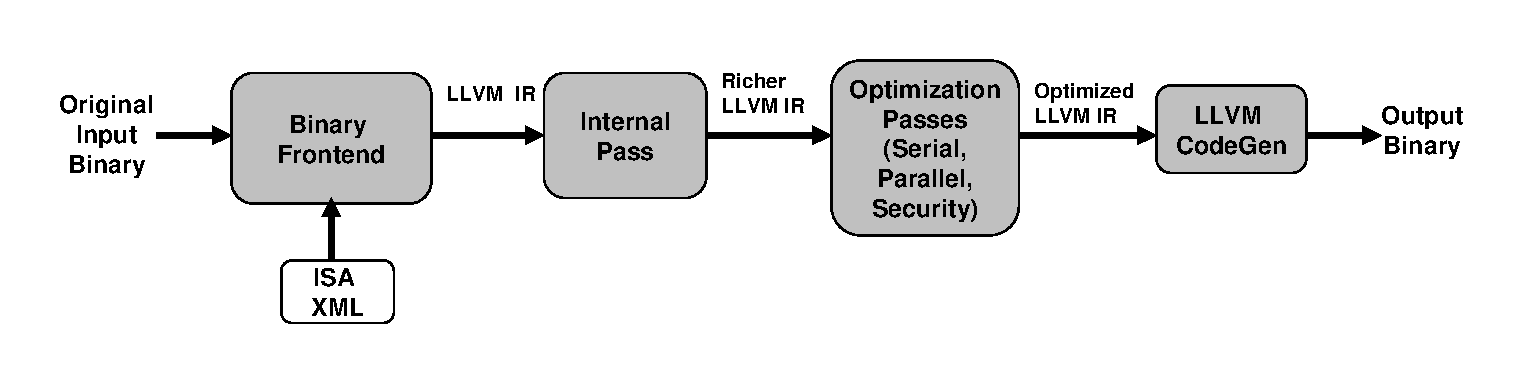
\includegraphics[scale=0.65]{sw_overview.eps}
\end{center}
\renewcommand{\baselinestretch}{1}
\small\normalsize
\begin{quote}
\caption{SecondWrite system}
\label{swoverview}
\end{quote}
\end{figure}
\renewcommand{\baselinestretch}{2}
\small\normalsize

The frontend module consists of a disassembler and a custom binary reader which processes the
individual instructions and generates an initial LLVM IR. This initial representation is void of the
desired IR features like function prototypes, abstract stack and virtual registers. The internal
pass module analyzes this initial IR to obtain an improved IR which has all the information and
features mentioned previously. Various optimization passes can be written on the above IR to obtain
an optimized IR. Finally, the optimized IR is passed to the existing LLVM code generator to obtain
the rewritten binary.

Various inherent characteristics of executables such as the unavailability of function prototypes,
the use of a phyiscal stack and the use of the set of phyiscal registers make it difficult to obtain
a high-level IR from an input executable. A number of techniques have been developed within our
group to extract this high-level information from executables whenever possible. We will not discuss
those techniques in this thesis as the techniques are explained in detail elsewhere \cite{}.

\section{Stack Canary Insertion}

The first component of our scheme is the simplest. LLVM provides the ability to insert stack
canaries during code generation. Utilizing this capability from LLVM allows us to easily provide the
same level of protection to an un-protected binary as StackGuard would provide when given an
application's source code.

Essentially, a random canary value is generated and placed on the stack during a function's prolog.
In the function epilog, the value stored on the stack is compared with the random canary value for
this process. If there is any difference, execution is halted as the canary value has been
corrupted.

While this component of our scheme is simple, it demonstrates a key advantage of SecondWrite. By
translating the input binary to LLVM's high-level intermediate representation, we were able to take
advantage of features LLVM already provides. Thus, to achieve the same level of protection as
StackGuard, we had to do very little once the binary was translated to LLVM's IR.

\section{Base Pointer Elimination}

The next component of our scheme is again due to existing LLVM optimizations. LLVM is an optimizing
compiler and the binaries produced by LLVM are highly optimized. One common optimization applied by
modern compilers on the x86 platform is to free up the EBP register for register allocation by
removing the base (or frame) pointer.

Eliminating the base pointer also removes the ability for an attacker to craft an attack by
modifying the old base pointer stored in a stack frame. In a binary which has not been compiled at a
high optimization level, base pointers may still be used. In this case, the value of the base
pointer will be pushed on the stack upon function entry in order for the value to be restored on
function return. If an attacker is able to modify the value of the base pointer, he/she could have a
fake stack frame they created be used thereby allowing the attacker to alter the flow of control of
the program.

When the base pointer is eliminated by LLVM, any attack of this form is immediately prevented. There
will be no base pointer for an attacker to modify. While corruption of the stack may still occur if
an attacker overflows a buffer in order to attempt to overwrite the base pointer, no attack will be
successful.

Again, the elimination of the base pointer highlights the advantages of SecondWrite. By utilizing an
existing compiler framework, we are able to produce highly optimized binaries which eliminate the
ability for an attacker to perform an attack on a base pointer.

\section{Return Address Protection}

Given that stack canaries as inserted by LLVM do not provide the same level of protection as the
ProPolice mechanism that comes with GCC, we decided to implement a more complete solution for
protecting against corruption of the return address.

The basic idea of our return address protection scheme is as follows:

\begin{enumerate}

 \item During the function prolog, store the return address of the current function in a global
 variable

 \item In function epilog, compare the current return address on the stack with the value saved in a
 global variable

 \item If there is any difference between these values, execution is halted

\end{enumerate}

This simple scheme will detect if the return address has been modified either directly or
indirectly. One complication with this scheme is the fact that a global variable is used for storing
the return address. If a separate global variable was created for each function, memory overhead
would become quite high. One solution is to use an array of global variables of a bounded size for
saving return values. However, if function nesting is deep as in recursive functions, issues can
still occur.

We applied an optimization for relieving this problem. We observed that this protection mechanism is
only necessary if a function contains a write to a buffer. Thus, we analyze a function to look for
any write to a buffer. If a function does not contain any write to a buffer then there is no need
for the return address protection mechanism to be inserted. During our experimental evaluation of
our scheme, we have not yet come across a recursive function, which could cause issues for our
scheme, that required return address protection to be inserted.

\section{Function Pointer Protection}

\section{longjmp/setjmp Protection}

%Appendix
\appendix
\renewcommand{\thechapter}{A}

\chapter{Overview}

The understanding of nonlinear processes in optical fibers is crucial towards 
extending the capabilities of modern optical communication systems based on 
wavelength division multiplexing (WDM), where each communication channel is 
represented by a unique wavelength. One of the nonlinear processes that 
limits the information carrying capacity of a WDM system is four-wave mixing 
(FWM), which causes cross-talk between neighboring channels. This places a 
lower limit on the wavelength separation between adjacent channels and an
upper limit on the input power in each channel. In this study, we describe
a process by which the evolution of FWM processes in an optical fiber can be 
used to estimate the inhomogeneities in the fiber core material, in particular 
the fluctuations in the linear refractive index of the fiber core.  

Experiments measuring the evolution of FWM processes along a length of fiber 
were carried out by Hart {\it et al.}\ \cite{hart1} and are described in detail in 
Sec.\ 2.2. In this experiment, two input pump waves at frequencies
$\omega_1$ and $\omega_2$, interacted with each other through the third-order 
nonlinearity of the fiber material to generate first-order sidebands at frequencies 
$\omega_3 = 2\omega_1 - \omega_2$ and $\omega_4 = 2\omega_2 - \omega_1$. 
These waves further interacted to produce second-order sidebands at 
$\omega_5 = 2\omega_3 - \omega_4$ and $\omega_6 = 2\omega_4 - \omega_3$. 
Higher-order sidebands were also generated. The normalized power in the 
sideband at frequency $\omega_m$ was represented by $\rho_m$. The 
evolution of the FWM processes was characterized by the evolution of 
$\rho_m$(z) as a function of fiber length z. 

In the present work, we make a quantitative comparison between these 
experimental results and our numerical results based on efficient algorithms 
\cite{Agrawal2} to solve the nonlinear Schr\"odinger equation (NLSE) that
governs the system. The numerical model, its underlying assumptions and
the results are described in Sec.\ 2.3. A realistic description of a 
standard single mode optical fiber must take into account the random phase 
perturbations a light wave undergoes while propagating through it, without 
disturbing the underlying conservative properties of the system. The NLSE 
needs to be suitably modified in order to incorporate the stochastic nature 
of the propagation. In order to preserve the conservative properties of the 
system, the stochastic terms in the NLSE must necessarily be multiplicative in 
nature as an additive term acts as a source or a sink. An algorithm that 
achieves this with linear, Gaussian, $\delta$-correlated noise is outlined in 
Sec.\ 2.3. This algorithm preserves the unconditional stability of the 
system. At the same time, care is taken to transform the stochastic NLSE from 
its original Ito representation \cite{ito} to the computationally feasible Stratanovich 
representation \cite{stratanovich} by compensating for the 
spurious linear drift that results from integrating such stochastic 
differential equations \cite{risken,werner2,drummond1,carter3}. The dominant 
sources of phase noise are discussed in Sec.\ 2.4. 

Conclusions on the relevance of the experiments of Hart {\it et al.}\ \cite{hart1} 
and the stochastic modeling presented here are summarized in Sec.\ 2.5.    

\section{Experimental and Computational Background}

In this work, we focus on tracing the evolution of the sidebands, generated 
through FWM, along a length of optical fiber. The FWM spectral evolution along
50\,m of fiber for two input pump power regimes (2.1\,W and 5.5\,W) was
investigated \cite{hart1}. In the 2.1\,W case, the sideband evolution followed a damped 
sinusoid along the length of the fiber. The experiments also found that the 
two first-order sidebands ($\rho_3$-blueshifted and $\rho_4$-redshifted from 
the two pumps) had different evolutions along the fiber (with different 
spatial wavelengths). For the 5.5\,W case, the evolution of both first- and 
second-order sidebands was measured. The damping in the first-order sidebands 
($\rho_3$ and $\rho_4$) occured faster than in the 2.1\,W case. Experiments 
probing the dependence of the sideband power on the input power (ranging from 
2\,W to 17\,W) were also performed at a fixed output length of 50\,m of the fiber.
At the same fiber length, the optical spectra for input powers ranging from 
2\,W to 17\,W were also recorded \cite{hart1}. The spectral envelopes were observed to fit 
well to a hyperbolic secant function and the fit parameters were recorded. 
Measurements with a high-resolution wavemeter showed that one of the two pumps 
consisted of two very closely spaced longitudinal modes 
($\Delta\nu\sim$ 0.5\,GHz) which were not resolved by the spectrometer used to 
record the FWM spectra. Inclusion of this multimode nature of the pump input 
in their model was found to alter the sideband dynamics dramatically and 
partly explained the asymmetry between the blue-shifted and red-shifted 
sidebands though it did not account for the damping in the sidebands. This 
was accounted for by adding weak phase fluctuations to the waves as they 
propagated along the fiber \cite{hart1}. The physical source of these phase fluctuations 
was not known at that time. However, the inclusion of the phase fluctuations 
into the model gave excellent qualitative and quantitative agreement with 
experiment. Their model involved integration of a system of coupled ODEs 
derived from the NLSE \cite{thompson1} by a process of truncation that 
retained only the leading frequency components (the pumps and the first- and 
second-order sidebands), a process justified by the fact that the input pump 
waves are well approximated by a combination of monochromatic waves. Their 
final numerical results are based on simulations using the truncated-ODE model
with Langevin noise terms representing phase fluctuations in the fiber. 
Another physical source of stochasticity in their experiment was the inherent 
power fluctuation in the lasers used as the input pumps. The level of 
fluctuations (5-20\%) was measured and incorporated appropriately into their 
model through stochastic initial conditions. This explained the evolution of 
the level of observed fluctuations in the sideband trajectories although it 
was found to be inadequate by itself, to account for the damping of the 
trajectories. They found that all three physical characteristics mentioned 
above, namely the multimode nature of the pump input, the stochastic phase 
fluctuations along the length of the fiber, and the stochastic initial power 
fluctuations were crucial to explaining the different features of the 
experimental measurements \cite{hart1}. 

\section{Stochastic NLSE Model}

In the present work, we have developed and implemented an unconditionally 
stable scheme for integrating the NLSE that successfully incorporates phase 
noise into the SSFM. Thus, we are now in a position to harness the high 
frequency / time resolution of the SSFM together with its efficient 
convergence properties. Due to these advances, we are now able to do 
simulations with much higher frequency resolution (60\,MHz as compared to 
300\,GHz in the ODE model). This high resolution, coupled with an appropriate 
convolution scheme, enables us to compare these simulated spectra with the 
composite spectra observed by the spectrometers which had a resolution of 
$\sim$ 60\,GHz. This was not possible with the truncated ODE model as the 
resolution of the simulated spectra in that case was $\sim$ 300\,GHz. For 
exactly the same levels of phase fluctuations, and initial condition 
fluctuations as used in Ref.\ \cite{hart1}, comparisons for the present NLSE 
model with the experimental sideband evolution functions $\rho_i(z)$ show 
excellent quantitative agreement. These results, along with the algorithms 
employed, are described in detail in this section. We have identified linear 
refractive index fluctuations along the fiber length to be a strong candidate 
for a physical source of the stochastic phase fluctuations. A comparison 
between the various possible sources is given in Sec.\ 2.4.

Under the assumption that the electric field of the light in the fiber has a 
slowly varying envelope $A(z,\tau)$, and that the fiber medium has an 
instantaneous nonlinear response, the system is well described by the 
nonlinear Schr\"{o}dinger equation (NLSE) with a linear multiplicative
stochastic term
%A.1
\begin{equation}
{\partial U \over \partial z} + {i\beta^{(2)} \over 2T_0^2} 
{\partial^2 U \over \partial\tau^2} + {\alpha U \over 2}
 + i\Gamma(z,\tau)U-i\gamma P_0 |U|^2 U = 0.
\end{equation}
$Z$ is distance along the length of the fiber, 
$U(z,\tau)=A(z,\tau)/\sqrt{P_0}$ is the complex electric field envelope 
$A(z,\tau)$ normalized to the absolute amplitude of the field $\sqrt{P_0}$, 
$P_0$ is the total power in the fiber, $\tau$ is time normalized to a 
convenient time scale $T_0(\sim 1\ ns)$ measured in a reference frame 
moving with the group velocity of the pulse [$\tau=(t-z/v_g)/T_0$]. The 
simulations are carried out for exactly the same physical parameters as the 
experiments and simulations reported by Hart {\it et al}.\ \cite{hart1}, i.e., 
$\beta^{(2)}=55\,(ps)^2/km$, is the group velocity dispersion of the fiber at 
the operating wavelength $\lambda_{0}\sim$ 632\,nm 
($k_0\sim 10^7\,m^{-1}$). A loss of $\sim$ 6\,dB/km gives $\alpha$ = 0.0014\,m$^{-1}$ as the 
loss in the fiber at this wavelength. The nonlinearity coefficient 
$\gamma=0.019\,W^{-1}m^{-1}$ is given by 
%A.2
\begin{equation}
\gamma = {\omega_{ave}n_2^I \over cA_{eff}},
\end{equation}
where $A_{eff}$ is the effective core area of the fiber,
$n_2^I$ is the Kerr coefficient for the intensity-dependent refractive index, and 
$\omega_{ave}$ is the average angular frequency of the wave envelope. 
$\Gamma(z,\tau)$ is a linear multiplicative phase noise field. In this study 
the noise field is assumed to be $\delta$-correlated in both space and time. 
The evolution of the FWM dynamics is found to be sensitive to the strength of 
this noise field. It can be physically interpreted as phase noise arising due 
to fluctuations in the linear refractive index of the fiber medium. A detailed 
discussion of its physical origin is given in Sec.\ 2.4.

The system was simulated using the Split-Step Fourier Method (SSFM) 
\cite{Agrawal2}. An algorithm for appropriately incorporating stochastic
phase fluctuations along the length of the fiber in the SSFM was developed
and is summarized below.

The NLSE is composed of linear and nonlinear terms, and can be written in operator form as
%A.3
\begin{eqnarray}
{\partial U \over \partial z} & = & (\hat{D}+\hat{S}+\hat{N})U \nonumber \\
\hat{D}& = & {-i\beta^{(2)} \over 2T_0^2}
{\partial^2 \over \partial\tau^2} - {\alpha \over 2} \nonumber \\
\hat{S} & = & i\Gamma(z,\tau) \nonumber \\
\hat{N} & = & i\gamma P_0|U|^2,
\end{eqnarray}
where $\hat{D}$, $\hat{S}$ and $\hat{N}$ are linear
(dispersive), nonlinear 
and stochastic operators, respectively. It has an exact solution for 
infinitesimal $\Delta z$ given by - 
%A.4
\begin{equation}
U(z + \Delta z,\tau) = exp[\Delta z(\hat{D} + \hat{S} + \hat{N})]U(z,\tau) ,
\end{equation}
which can be approximated by
%A.5
\begin{equation}
U(z + \Delta z,\tau) \approx exp[\Delta z \hat{D}]exp[\Delta z \hat{S}]exp[\Delta z \hat{N}]U(z,\tau) .
\end{equation}

The execution of $exp[\Delta z \hat{N}]$ is carried out in $\tau$-space:
%A.6
\begin{equation}
B_1(z,\tau)=exp[\Delta z \hat{N}]U(z,\tau) .
\end{equation}

The execution of $exp[\Delta z \hat{S}]$ and $exp[\Delta z \hat{D}]$ is 
carried out in $\omega$-space.

In particular, the stochastic phase fluctuations are introduced by modifying 
the phase $\phi_j$ of each frequency component $\omega_j$ of the complex 
field according to
%A.7
\begin{eqnarray}
B_2(z,\omega) & = & {\cal{F}}[B_1(z,\tau)] \nonumber \\
B_3(z,\omega_{j}) & = & exp[i \delta\phi(z,\omega_j)]B_2(z,\omega_j) ,
\end{eqnarray}
where $\cal{F}$ represents the Fourier transform operation.

This process only modifies the phase of each complex frequency component, 
leaving its absolute value unchanged. Thus the algorithm conserves the total 
power and the unconditional stability of the system.

The stochastic phase fluctuations $\delta\phi(z,\omega_j)$ are taken to be 
$\delta$-correlated in frequency as well as spatially along the fiber length. 
The Box-Muller algorithm \cite{boxmuller} was used to generate Gaussian random
deviates from computer-generated uniform random deviates $r_{1j}$ and $r_{2j}$
at each spatial step and for each frequency component $\omega_j$. The 
fluctuations are given by
%A.8
\begin{equation}
\delta\phi(z,\omega_{j}) = \sqrt{-2\sigma_{\phi}^2 \Delta z ln(r_{1j})}cos(2 \pi r_{2j}) .
\end{equation}

This is followed by the execution of $exp[\Delta z \hat{D}]$, which is also 
carried out in Fourier space, followed by the inverse transform
%A.9
\begin{equation}
U(z + \Delta z,\tau) = {\cal{F}}^{-1}[exp[\Delta z \hat{D}(i\omega)]B_{3}(z,\omega)] .
\end{equation}

$\hat{D}(i\omega)$ is obtained by replacing $(\partial / \partial \tau)$ 
by $i \omega$.

%Figure A.1
\begin{figure}
\begin{center}
\includegraphics[0in,0in][3.25in,4.266in]{nlsetime.eps}
\end{center}
\renewcommand{\baselinestretch}{1}
\small\normalsize
\begin{quote}
\caption{Multimode pulse input to the NLSE: (a) input pulse in time
domain and (b) input spectrum.}
\label{figA.1}
\end{quote}
\end{figure}
\renewcommand{\baselinestretch}{2}
\small\normalsize

The basic form of the initial complex wave envelope function is 
%A.10
\begin {equation}
U(0,\tau) = exp \left( - {\tau^2 \over 2\tau_p^2} \right)
\left\{ 
\begin{array}{l}
exp\left( {i\Omega\tau \over 2} \right) + \\
exp\left( - {i\Omega\tau \over 2} \right)
\end{array}
\right\} ,
\end{equation}
where $\tau_p$ is the pulse width T$_p$ =5\,ns FWHM, normalized to the time scale 
T$_0$, $\Omega$=366\,GHz is the frequency detuning between the two laser 
sources normalized to a frequency scale $\Omega_0$ = 62.5\,MHz.  Figure A.1(a) 
shows a plot of this pulse $|U(0,\tau)|^2$. The overall Gaussian envelope 
has an FWHM of 5\,ns, the closely spaced dark lines are due to the 366\,GHz 
($\sim$3\,ps) beating between the two input pump frequencies. The 2\,ns 
modulations on the pulse are due to the 0.5\,GHz mode-structure in the 
blue-shifted pump wave. Figure A.1(b) shows the input spectrum of this pulse 
which consists of two highly monochromatic pump waves with a detuning of 
$\Omega$=366\,GHz. The spectrum of the blue-shifted pump, upon magnification, 
is seen to be composed of two very closely spaced peaks, with a separation of 
$\Delta\nu$=0.5\,GHz. Hart {\it et al}.\ \cite{hart1} did not use pulsed 
wave functions in their NLSE simulations as the size of the FFT required to do 
so made it computationally prohibitive at that time. The size of the FFT was 
chosen such that it would accommodate a time span of 16\,ns in order to go 
sufficiently far into the wings on the Gaussian pulse; and a frequency span of 
16\,THz in order to accommodate all the sidebands generated and prevent 
spurious effects due to the reflection boundary conditions implicit in the 
SSFM algorithm. These considerations dictated the size of the FFT to be 
$\geq$(16 THz)$\cdot$(16 ns) = 256000. The nearest power of 2 is 
2$^{18} = 262144$, which has been used throughout the present work. The 
incorporation of the pulsed nature of the light was found to be necessary in 
explaining the dynamics. From the perspective of the coupled amplitude 
equations used by Hart {\it et al}.\ \cite{hart1}, the present model is equivalent 
to a coupled-ODE model with $2^{18}$ coupled ODEs. 

%Figure A.2
\begin{figure}
\begin{center}
\includegraphics[0in,0in][6in,4.572in]{modestruc21ornot.eps}
\end{center}
\renewcommand{\baselinestretch}{1}
\small\normalsize
\begin{quote}
\caption[Short caption for Figure A.2.]
{Effects of inclusion of the multimode nature ($\Delta\nu = 0.5$\,GHz) of the blue-shifted input pump laser on the 1st order sideband evolution as a function of fiber length for P$_0 = 2.1$\,W. Dashed curves represent simulations without the multimode nature and solid curves represent simulations with the multimode nature. $\Omega = 366$\,GHz, $\gamma = 0.019$\,W$^{-1}$\,m$^{-1}$, and $\beta^{(2)} = 55$\,ps$^2$/km (a) power in the blue-shifted sideband, (b) power in the red-shifted sideband.}
\label{figA.2}
\end{quote}
\end{figure}
\renewcommand{\baselinestretch}{2}
\small\normalsize

%Figure A.3
\begin{figure}
\begin{center}
\includegraphics[0in,0in][6in,4.572in]{modestruc55ornot.eps}
\end{center}
\renewcommand{\baselinestretch}{1}
\small\normalsize
\begin{quote}
\caption[Effects of inclusion of the multimode nature]
{Effects of inclusion of the multimode nature ($\Delta\nu = 0.5$\,GHz) of the blue-shifted input pump laser on the 1st order sideband evolution as a function of fiber length for P$_0 = 5.5$\,W. Dashed curves represent simulations without the multimode nature and solid curves represent simulations with the multimode nature. $\Omega = 366$\,GHz, $\gamma = 0.019$\,W$^{-1}$\,m$^{-1}$, and $\beta^{(2)} = 55$\,ps$^2$/km (a) power in the first-order blue-shifted sideband, (b) power in the first-order red-shifted sideband, (c) power in the second-order blue-shifted sideband, (d) power in the second-order red-shifted sideband.}
\label{figA.3}
\end{quote}
\end{figure}
\renewcommand{\baselinestretch}{2}
\small\normalsize

%Figure A.4
\begin{figure}
\begin{center}
\includegraphics[0in,0in][6in,4.572in]{nlsez21cwpulse.eps}
\end{center}
\renewcommand{\baselinestretch}{1}
\small\normalsize
\begin{quote}
\caption[Effects of inclusion of the pulsed nature]
{Effects of inclusion of the pulsed nature (5\,ns FWHM) of the input pump laser light on the first-order sideband evolution as a function of fiber length for P$_0 = 2.1$\,W. Dashed curves represent cw simulations and solid curves represent pulsed simulations. $\Omega = 366$\,GHz, $\Delta\nu = 0.5$, $\gamma = 0.019$\,W$^{-1}$m$^{-1}$, and $\beta^{(2)} = 55$\,ps$^2$/,km (a) power in the blue-shifted sideband, (b) power in the red-shifted sideband.}
\label{figA.4}
\end{quote}
\end{figure}
\renewcommand{\baselinestretch}{1}
\small\normalsize

%Figure A.5
\begin{figure}
\begin{center}
\includegraphics[0in,0in][6in,4.572in]{nlsez55cwpulse.eps}
\end{center}
\renewcommand{\baselinestretch}{1}
\small\normalsize
\begin{quote}
\caption
[Other effects of inclusion of the pulsed nature]
{Effects of inclusion of the pulsed nature (5\,ns FWHM) of the input pump laser on the first- and second-order sideband evolution as a function of fiber length for P$_0 = 5.5$\,W. Dashed curves represent cw simulations and solid curves represent pulsed simulations. $\Omega = 366$\,GHz, $\Delta\nu = 0.5$, $\gamma = 0.019$\,W$^{-1}$m$^{-1}$, and $\beta^{(2)} = 55$\,ps$^2$/,km (a) power in the first-order blue-shifted sideband, (b) power in the first-order red-shifted sideband, (c) power in the second-order blue-shifted sideband, (d) power in the second-order red-shifted sideband.}
\label{figA.5}
\end{quote}
\end{figure}
\renewcommand{\baselinestretch}{2}
\small\normalsize

Upon incorporation of the multimode nature of the blue input pump laser source 
and the stochastic fluctuations in the initial power in the lasers, the 
initial wave function takes the form
%A.11
\begin {equation}
U(0,\tau) = exp\left( - {\tau^2 \over 2\tau_p^2} \right)
\left\{
\begin{array}{l}
\sqrt{{1 + \delta\rho_1 \over 2}} 
\left[ \begin{array}{l}
exp \left( {i(\Omega+\Delta\nu)\tau \over 2} \right) + \\
exp \left( {i(\Omega-\Delta\nu)\tau \over 2} \right) 
\end{array} \right]\\
+ \sqrt{1 + \delta\rho_2} exp\left( - {i\Omega\tau \over 2} \right)
\end{array}
\right\}.
\end{equation}

\

\noindent $\Delta\nu = 0.5$\,GHz is the frequency separation between the two longitudinal 
modes in the blue-shifted pump. $\delta\rho_1$ and $\delta\rho_2$ are 
Gaussian random deviates (generated using the Box-Muller algorithm 
\cite{boxmuller}) that represent the initial power fluctuations in each of the 
pump laser sources. Their standard deviations were taken to be, 
$\sigma_{\rho_1} = 0.2$, $\sigma_{\rho_2} = 0.11$ for simulations from 0\,m to 
20\,m, $\sigma_{\rho_1} = 0.12$, $\sigma_{\rho_2} = 0.05$ for simulations from 
20\,m to 50\,m along the length of the fiber. This is exactly the same 
prescription used by Hart {\it et al}.\ \cite{hart1} in their simulations and is 
dictated by their experimental measurements of the fluctuations in the pump 
laser intensities.

At this point it is worth noting the effects of the inclusion of two attributes of 
the input laser light, namely, the multimode nature of the blue-shifted pump, and 
the pulsed nature of the input light (assumed to be cw in the simulations reported by 
Hart {\it et al}.\ \cite{hart1}). 

Figure A.2 shows a comparison between simulations with (solid curves) and without (dashed curves) the multimode nature for an input pump power of 2.1 Watts. The simulations with the mode structure show the asymmetry between the blue- and red-shifted sideband evolution, in particular, the difference in spatial wavelength between the two, and a non-return to zero nature of the evolution, as observed in the experimental data (black dots with error bars). These features are absent in the simulations without mode-structure. $\rho_3$ and $\rho_4$ stands for the first order blue- and red-shifted sidebands respectively.  Figure 2.3 shows the corresponding comparison for the case of 5.5 Watts of input pump power.  Here, too, the simulations incorporating the multimode nature of the blue-shifted pump (solid curves) are seen to be an improvement over those not incorporating it (dashed curves). A feature of the experimental data (black dots with errorbars) is that for the $\rho_3$ sideband, the initial part of the evolution involves a peak followed by a shoulder, while for the $\rho_4$ sideband, the initial part of the evolution involves a shoulder followed by a peak. This feature, too, is seen to occur as a result of the inclusion of the multimode nature of the blue-shifted pump.  

The effect of inclusion of the pulsed nature of the input beam is seen in Fig.\ A.4 (for the 2.1 Watt case) and Fig.\ A.5 (for the 5.5 Watt case). The solid dashes represent simulations for a cw input beam and the solid curves represent those for a pulsed input beam. The incorporation of the pulsed nature clearly results in damping of the sideband trajectories which are seen to come closer to the experimental data \cite{hart1} (black dots with error bars). 

Use of the FFT algorithm makes evaluation relatively fast compared to other 
finite-difference schemes. The computational error is $O(\Delta z^2)$, thus 
the solution converges with decreasing spatial step-size $\Delta z$. 

The simulations were tested for the conservation of total power along the 
fiber length (by setting the loss $\alpha$ to zero) and for the conservation 
of asymmetry \cite{thompson1,hart1} given by 
%A.12
\begin{equation}
C(Z) = \sum_{i=1}^{\infty}(2i-1)[\rho_{2i-1}(Z)-\rho_{2i}(Z)] .
\end{equation}

A clearer picture of the evolution of the sidebands is obtained by plotting both the 
power in the sidebands and their standard deviations as a function of length along the fiber. Figures A.6(a) and A.6(b) show a comparison between simulation and experiment of the evolution 
of the first-order blue-shifted ($\rho_3$) and red-shifted ($\rho_4$) sidebands,  
respectively, for an input power of 2.1 W. The dashed curves represent NLSE simulations 
which include the stochastic nature of the input powers of the pump lasers but exclude 
the stochastic phase fluctuations added along the length of the fiber, an attribute 
which is included in the simulations represented by the solid curves. The black dots 
with error bars represent the experimental data. The measured sideband 
power, normalized to the total power in the fiber, is periodic in length but 
appears to be damping to a constant value. The measured data also show a clear 
difference between the spatial wavelengths of oscillation of the blue-shifted ($\rho_3$) and red-shifted ($\rho_4$) sidebands trajectories, respectively. Both these features are captured well by both the simulations. Figures A.6(c) and A.6(d) compare experimental and simulated 
measures of the evolution of the standard deviation in the sideband power 
along the fiber length. It is clearly observed that simulations with phase noise 
added to the light field along the length of the fiber (solid curves) are closer to the 
experimental data as compared to those that exclude this feature (dashed curves). This indicates
the instrumental nature of the phase fluctuations in explaining key features of the dynamics.

%Figure A.6
\begin{figure}
\begin{center}
\includegraphics[0in,0in][6in,4.572in]{nlsez21phaseornot.eps}
\end{center}
\renewcommand{\baselinestretch}{1}
\small\normalsize
\begin{quote}
\caption
[Comparison between experiments measurements]
{Comparison between the experimental measurements \cite{hart1}(black), the random initial condition NLSE model excluding phase noise (dashed curves) and the stochastic phase noise NLSE model (solid curves) showing the first-order sideband evolution as a function of fiber length for P$_{0} = 2.1$\,W, $\Omega = 366$\,GHz, $\Delta\nu = 0.5$\,GHz,$\gamma = 0.019$\,W$^{-1}$m$^{-1}$, and $\beta^{(2)} = 55$ps$^2$/km: dynamical evolution of the: (a) power in the blue-shifted sideband, (b) power in the red-shifted sideband, (c) fluctuations in the blue-shifted sideband, (d) fluctuations in the red-shifted sideband.}
\label{figA.6}
\end{quote}
\end{figure}
\renewcommand{\baselinestretch}{2}
\small\normalsize

The apparent damping of the periodic sideband trajectory is seen more 
dramatically in Figs.\ A.7(a) and A.7(b), which show the evolution of the 
first-order sideband power along the fiber for an input power of 5.5\,W. 
The two first-order sidebands evolve differently. They appear to 
damp to a constant value at a faster rate than for the case with an input pump 
power of 2.1\,W. Here again, NLSE simulations that incorporate phase noise along the length
of the fiber (solid curves) are much more successful in accurately capturing the dynamical features of the system than NLSE simulations that do not take this feature into account (dashed curves).  Figures A.7(c) and A.7(d) show a comparison between the simulated and measured standard deviations. Comparisons for the second-order blue-shifted ($\rho_5$) and red-shifted ($\rho_6$) sidebands, respectively, are shown in Figs.\ A.7(e) and A.7(f). 


%Figure A.7
\begin{figure}
\begin{center}
\includegraphics[0in,0in][6in,4.572in]{nlsez55phaseornot.eps}
\end{center}
\renewcommand{\baselinestretch}{1}
\small\normalsize
\begin{quote}
\caption
[This figure caption is indented and single-spaced.]
{This figure caption is indented and single-spaced.  Comparison between the experimental measurements \cite{hart1} (black), the random initial condition NLSE model excluding phase noise (dashed curves) and the stochastic phase noise NLSE model (solid curves) showing the first- and second-order sideband evolution as a function of fiber length for P$_{0} = 5.5$\,W, $\Omega = 366$\,GHz, $\Delta\nu = 0.5$\,GHz, $\gamma = 0.019$\,W$^{-1}$m$^{-1}$, and $\beta^{(2)} = 55$\,ps$^2$/km: dynamical evolution of the: (a) power in the first-order blue-shifted sideband, (b) power in the first-order red-shifted sideband, (c) fluctuations in the first-order blue-shifted sideband, (d) fluctuations in the first-order red-shifted sideband, (e) power in the second-order blue-shifted sideband, (f) power in the second-order red-shifted sideband.}
\label{figA.7}
\end{quote}
\end{figure} 
\renewcommand{\baselinestretch}{2}
\small\normalsize

The observed dynamical evolution of the sidebands is found to depend 
sensitively on the strength of the stochastic phase fluctuations. Yet, best 
agreement with the experimental results of Hart {\it et al}.\ \cite{hart1} is 
achieved with exactly the same noise strength $\sigma^2_\phi$ as used in 
their truncated ODE model, namely, $\sigma^2_\phi = 0.0067$\,m$^{-1}$. They 
report that including phase noise in their FWM calculations resulted in a 
spurious linear drift in the trajectories for the sideband power with length. 
To remove this artifact of the computations, they added a linear loss to their 
coupled ODEs. They set the loss coefficient $\alpha = 0.0046$\,m$^{-1}$ by 
finding the value that removed this increasing slope. We have observed exactly 
the same secular growth phenomenon for a wide range of the noise strength 
$\sigma^2_\phi$ and have arrived at an empirical prescription for $\alpha$ 
namely, $\alpha\sim\sigma^2_\phi$, where $\sigma^2_\phi$ is the 
variance of the added phase noise. This indicates the general nature of 
dynamics resulting from the addition of stochastic, $\delta$-correlated phase 
fluctuations to systems governed by nonlinear partial differential equations 
\cite{risken}. 

It is remarkable that the strength of the phase noise required is the same in 
both the 2.1\,W and the 5.5\,W cases. Further, it is worth noting that exactly 
the same noise strength was used by Hart {\it et al}.\ \cite{hart1}, the difference 
being that they introduced phase noise only in the pump frequencies, whereas 
we have introduced it in all the Fourier modes ($\sim2^{18}$). As a 
confirmation of this result, they also performed experiments and numerical 
simulations examining the sideband power dependence on the input power at a 
fixed length of 50.4\,m of the same fiber. We have repeated these simulations 
with the stochastic NLSE model and the results are shown in Figs.\ 2.8(a) 
(blue-shifted sideband) and 2.8(b) (red-shifted sideband). The experimental 
measurements of the sideband powers are represented by filled squares and the 
results of numerical simulations are represented by triangles (without phase 
noise) and by circles (with phase noise). The simulations are seen to follow 
the general trend seen in the experiments. As the pump power is increased, the 
triangles (without phase noise) start to disagree with experiment, whereas the 
circles (with phase noise) are much closer to experiment. The phase noise 
strength used in these simulations was exactly the same as that used in the 
simulations depicted in Figs.\ A.6 and A.7. The agreement between the phase noise 
simulations and the experimental data was (once again) highly sensitive to the 
noise strength. Since this experiment (unlike those shown in Figs.\ A.2 - A.7) 
is non-destructive, it can be used to deduce the strength of phase noise 
processes in a given optical fiber. It will be shown in Sec.\ 2.4 that a 
likely cause of the phase noise is fluctuation in the linear refractive index 
of the fiber. The noise strength deduced from the present computational study 
corresponds to a refractive index inhomogeneity of 
$\langle \Delta n^{2} \rangle \sim 10^{-16}$.   

%Figure A.8
\begin{figure}
\hspace{1.25in}
\includegraphics[0in,0in][6in,4.572in]{nlsefinal.eps}
\renewcommand{\baselinestretch}{1}
\small\normalsize
\begin{quote}
\caption
[Comparison between the experiments measurements (filled squares]
{Comparison between the experimental measurements (filled squares), simulations without stochastic phase fluctuations (open triangles) and with stochastic phase fluctuations (open circles) of the first-order sideband power versus pump input power for L=50.39\,m, and $\Omega = 366$\,GHz: power in the (a) blue-shifted sideband and (b) red-shifted sideband.}
\label{figA.8}
\end{quote}
\end{figure}
\renewcommand{\baselinestretch}{2}
\small\normalsize

%Figure A.9
\begin{figure}
\begin{center}
\includegraphics[0in,0in][6in,4.572in]{fig292.eps}
\end{center}
\renewcommand{\baselinestretch}{1}
\small\normalsize
\begin{quote}
\caption
[Evolution of the FWM spectrum]
{Evolution of the FWM spectrum along the fiber (a) P=2.1\,W, experiment, (b) P=5.5\,W, experiment, (c) P=2.1\,W, stochastic-NLSE model, (d) P=5.5\,W, stochastic-NLSE model.}
\label{figA.9}
\end{quote}
\end{figure}
\renewcommand{\baselinestretch}{2}
\small\normalsize

Till now the comparisons between our simulations of the full NLSE and the 
truncated ODE model give basically the same results, although with much better 
agreement with experiment. However, the full NLSE can also provide a detailed 
comparison with the experimental spectra. This was not available from the 
truncated ODE model. The simulations reported in this work were carried out 
with a very high frequency and time resolution in order to incorporate the 
fact that the input light was not cw, but was composed of $\sim$ 5\,ns long 
pulses; and that the number of sidebands generated required the frequency 
spread of the FFT to be $\sim$ 16\,THz, while resolving a longitudinal 
mode-structure of $\Delta\nu$ $\sim 0.5$\,GHz. The spectral resolution used was 
$\sim$ 0.05\,GHz, whereas the spectrometer used to observe the spectra had a 
resolution 1000 times larger ($\sim$ 50\,GHz). To account for this difference, 
the simulated spectra were first convolved with a Gaussian of unit peak and 
62\,GHz FWHM, before they were compared with the observed spectra.  

Figures A.9(a) and A.9(b) show three-dimensional plots of the average experimental 
FWM output spectrum along the length of the fiber for input pump powers of 2.1\,W and 5.5\,W,
 respectively (courtesy Hart {\it et al}.\ \cite{hart1}). The vertical 
axis represents the intensity, normalized to the peak power in one of the 
input pumps, plotted on a logarithmic scale. The pump frequencies are centered 
on $+/-\Omega/2$ and the fiber length is increasing into the page. Figures 
9(c) and 9(d) show the corresponding comparisons based on simulations using 
the stochastic-NLSE model. The basic features of the spectral evolution are 
captured by the simulations. 

%Figure  A.10
\begin{figure}
\begin{center}
\includegraphics[0in,0in][6in,4.573in]{nlsespec.eps}
\end{center}
\renewcommand{\baselinestretch}{1}
\small\normalsize
\begin{quote}
\caption
[Experimental FWM output spectrum]
{Experimental FWM output spectrum (solid line), convolved spectra from simulations of the stochastic NLSE model (dashed line), and hyperbolic secant envelope fit (dotted line) for pump input powers P$_0$ of (a) 2.1\,W, (b) 5.5\,W, (c) 6.7\,W, (d) 8.3\,W, (e) 12.7\,W, (f) 17.4\,W, fiber length L$= 50.39$\,m, $\Omega = 366$\,GHz, $\Delta\nu = 0.5$\,GHz, $\gamma = 0.019$\,W$^{-1}$m$^{-1}$, and $\beta^{(2)} = 55$\,ps$^2$/km.}
\label{figA.10}
\end{quote}
\end{figure}
\renewcommand{\baselinestretch}{2}
\small\normalsize

Hart {\it et al}.\ \cite{hart1} also documented the experimentally observed FWM 
output spectra for a fixed fiber length of 50.39 meters for 6 different input 
pump powers. They state the coefficients A and B of the hyperbolic secant 
envelopes that best fit the output spectra which are given by
%A.13
\begin{equation}
f(\omega) = Asech(B\omega) ,
\end{equation}
where A and B are the experimental fit parameters.

The hyperbolic secant parameters A and B, that best fit the simulated spectra 
are exactly the same as those that best fit the experimental spectra 
\cite{hart1} for all the 6 cases of input power considered. Figure 2.10 shows an 
overlap of the simulated spectra (dashed line), with the experimental spectra 
(solid line) and the experimental hyperbolic secant envelope (dotted line) for 
6 different pump powers, namely, (a) 2.1\,W, (b) 5.5\,W, (c) 6.7\,W, (d) 8.3\,W, (e) 
12.7\,W, (f) 17.4\,W. The hyperbolic secant parameters for each of these pump 
powers are (a) A=3.85 and B=0.36, (b) A=2.26 and B=0.27, (c) A=1.81, B=0.25, 
(d) A=1.56 and B=0.23, (e) A=0.98,B=0.20, and (f) A=0.81 and B=0.20. The exact 
shapes of the simulated spectra match very well with the experimental spectra 
for low input pump powers (2.1\,W and 5.5\,W), but tend to lack the "filled-in" 
character of the experimental spectra at higher powers (6.7\,W, 8.3\,W, 12.7\,W and 
17.4\,W).

\section{Discussion}

Hart {\it et al}.\ \cite{hart1} postulated that strong candidates for the possible 
physical sources of the phase fluctuations are stimulated Brillouin 
scattering, stimulated Raman scattering and fiber medium inhomogeneities. 
Brillouin scattering was eliminated as a source, since a backward propagating 
wave, which is a signature of Brillouin scattering in optical fibers, was not 
observed in the experiments. We have  modeled stimulated Raman scattering 
\cite{Agrawal8, headley} for our system and have found no evidence to
support the hypothesis that it could be a possible source of the stochastic phase 
fluctuations for fiber lengths up to 50 meters and pump power levels up to 5.5 Watts. 
A more detailed discussion of the Raman scattering simulations performed is given in Chap.\ 3.
Apart from these, quantum phase fluctuations are another well 
known, though extremely weak, source of phase noise in optical fibers 
\cite{Agrawal2,perlmutter1}.

Fiber medium inhomogeneities were identified as the major cause of the 
stochastic phase fluctuations. These inhomogeneities can manifest themselves 
through spatial and/or temporal fluctuations in the fiber parameters, namely, 
the linear refractive index $n_0$, the group velocity $v_g$, the group 
velocity dispersion $\beta^{(2)}$ and the nonlinearity 
$\gamma$ \cite{abdullaev}. Of these, the fluctuation in the linear refractive 
index was found to be the only source of phase fluctuation that had a 
significant effect on the dynamics. A relationship between the level of 
refractive index fluctuations and the  corresponding level of phase 
fluctuations has been arrived at. It is found that refractive index 
fluctuations as small as $\sigma_n^2 \sim 10^{-17}$\,m$^{-1}$ can cause the 
desired phase fluctuations. Possible sources of these refractive index 
fluctuations are discussed below.   

Consider the modified nonlinear Schr\"odinger equation (NLSE) which is
stated below, with the linear multiplicative noise term represented in terms of 
spatial and temporal fluctuations in the refractive index of the fiber.
%A.14
\begin{equation}
{\partial U \over \partial z} + {i\beta^{(2)} \over 2T_0^2} {\partial^2U \over \partial\tau^2} + {\alpha U \over 2} + ik_0 \delta n(z,\tau)U - i\gamma P_{0}|U|^2 U = 0 ,
\end{equation}
where $\delta n(z,\tau)$ is the spatial and temporal variation of the refractive 
index along the fiber. It can be caused by temperature and density 
fluctuations in the fiber \cite{glenn}. 

The thermodynamic estimate for $\Delta n$ is given by \cite{glenn}
%A.15
\begin{equation}
\langle \Delta n^{2} \rangle = {-kT\rho^2 \over V^2}  
\left( {\partial V \over \partial P} \right)_{T} 
\left( {\partial n \over \partial \rho} \right)_{T}^{2}
 + {kT^2 \over \rho VC_v} \left( {\partial n \over \partial T} \right)_{\rho}^2 .
\end{equation} 

This gives the mean-square index fluctuation in terms of the properties of 
the material. It can be rewritten as
%A.16
\begin{equation}
\langle \Delta n^{2} \rangle = {V_{\rho}+V_T \over V} = \langle \Delta n^{2} \rangle_{\rho}+\langle \Delta n^{2} \rangle_{T} .
\end{equation}

For a fiber of length z=1\,m and radius r=2.82\,$\mu$m 
(Volume V=2.5 $\times 10^{-12}$\,m$^3$), these have been calculated to be 
%A.17
\begin{eqnarray}
\langle \Delta n^2 \rangle_{\rho} \sim 10^{-21} & \equiv & \langle \Delta \rho^2 \rangle \sim 10^{-14} 
{kg^2 \over m^6}, \nonumber \\
\langle \Delta n^2 \rangle_T \sim 10^{-23} & \equiv & \langle \Delta T^2 \rangle \sim 10^{-12}~{^\circ}C^2 .
\end{eqnarray}

It should be noted that $\langle \Delta n^2 \rangle \propto (1/z) \Rightarrow \delta n \propto  (1 / \sqrt{z})$. The corresponding phase fluctuation that this would lead to in the NLSE is given by $\delta \phi=k_{0} \delta n z \propto \sqrt {z}$, which is equivalent to the prescription for incorporating phase fluctuations into the stochastic NLSE model described in Sec.\ 2.3, namely,  $\langle \Delta \phi^2 \rangle = 6.7 \times 10^{-3}z$. Hart {\it et al}.\ \cite{hart1} used the same prescription and the same noise strength in their truncated-ODE model. From this we can estimate the level of refractive index fluctuation that corresponds to the noise strength used in the simulations described in Sec.\ 2.3 
%A.18
\begin{eqnarray}
\langle \Delta n^2 \rangle = {6.7 \times 10^{-3} \over k_0^2} = 6.78 \times 10^{-17} \nonumber\\
\equiv \langle \Delta T^{2} \rangle \sim 10^{-6}~{^\circ}C^2 \equiv \Delta T \sim 10^{-3}~{^\circ}C 
\end{eqnarray}

The temperature coefficient of the refractive index of silica \cite{glenn}, 
$(\partial n / \partial T)_{\rho} \sim 10^{-5} ~{^\circ}C^{-1}$. Thus even small spatio-temporal temperature fluctuations of $\sim 10^{-3} ~{^\circ}C$ are enough to cause the inferred level of refractive index fluctuations.

The refractive index fluctuations could also be due to inhomogeneities in the 
density of the fiber material, frozen in at the time of manufacture of the 
fiber. The simulations were averaged over $\sim$ 600 iterations to get a good 
estimate of the power fluctuations in the sidebands. Initially, simulations 
were performed with a different phase noise distribution for each iteration. 
Later, a particular (arbitrary) phase noise distribution was selected and 
frozen for all the iterations.
This did not reduce the level of damping observed in the sideband trajectories 
provided that the strength of the phase noise was kept the same, thus 
indicating that density fluctuations induced during fiber manufacture could be 
a possible source. The phase noise was modeled as $\delta$-correlated in
both space and time. A more realistic approach would be to use correlated
noise. Numerical methods to incorporate linear multiplicative correlated noise 
into the NLSE have been developed by M.J. Werner {\it et al}.\ \cite{werner2}.

\section{Conclusions}

The role of stochasticity in the dynamical evolution of four-wave-mixing 
processes in an optical fiber has been investigated. This research consisted 
of theoretical and numerical computations. It focuses on tracing the evolution 
of the sidebands, generated through FWM, along a length of optical fiber. 
Detailed comparisons were made with the experimental results of 
Hart {\it et al}.\ \cite{hart1} and the agreement was excellent. The present work 
uses numerical techniques that have much higher resolution and better 
efficiency, and it presents a theoretical basis for the role of the 
stochasticity in the dynamics. The system is known to be governed by the 
nonlinear Schr\"odinger equation (NLSE) to a very good 
approximation \cite{Agrawal2}. 

A powerful technique that can be used for simulations of the stochastic NLSE 
is the Split-step Fourier Method (SSFM) \cite{Agrawal2}. An algorithm for the 
direct implementation of stochastic processes along the length of the fiber in 
the SSFM has been developed. The advantages of this approach with respect to 
the coupled-ODE approach are that we can carry out simulations with much 
higher frequency and time resolution without sacrificing computational 
efficiency.
 
The physical sources of these stochastic phase fluctuations are investigated 
quantitatively and are identified to be due to fluctuations in the linear 
refractive index of the fiber. Strong candidates for the causes of these 
refractive index fluctuations are temperature fluctuations in the fiber medium 
caused by the fluctuating temperature of the fiber environment, density 
fluctuations in the fiber medium frozen into the fiber during manufacture, and 
intrinsic thermodynamic fluctuations in the temperature and density of the 
fiber.  

The experiments performed by Hart {\it et al}.\ \cite{hart1} can be used to 
determine the level of these refractive index fluctuations in commercial 
fibers. Results described in Figs.\ 2 and 3 represent a destructive 
experiment that measures the sideband evolution with fiber length for a fixed 
input pump power, necessarily requiring the fiber to be cut repeatedly. The 
level of refractive index fluctuations can be used as a parameter in the 
simulations to best fit the experimental results. Alternatively, Fig.\ 4 
represents a non-destructive experiment that measures the sideband evolution 
with input pump power for a fixed fiber length. These experiments are found to 
be effective for estimating the refractive index fluctuations, as the dynamics 
is observed to be sensitively dependent on the strength of the phase 
fluctuations. 


%Appendix

\renewcommand{\thechapter}{B}

\chapter{Overview}

The understanding of nonlinear processes in optical fibers is crucial towards 
extending the capabilities of modern optical communication systems based on 
wavelength division multiplexing (WDM), where each communication channel is 
represented by a unique wavelength. One of the nonlinear processes that 
limits the information carrying capacity of a WDM system is four-wave mixing 
(FWM), which causes cross-talk between neighboring channels. This places a 
lower limit on the wavelength separation between adjacent channels and an
upper limit on the input power in each channel. In this study, we describe
a process by which the evolution of FWM processes in an optical fiber can be 
used to estimate the inhomogeneities in the fiber core material, in particular 
the fluctuations in the linear refractive index of the fiber core.  

Experiments measuring the evolution of FWM processes along a length of fiber 
were carried out by Hart {\it et al.}\ \cite{hart1} and are described in detail in 
Sec.\ 2.2. In this experiment, two input pump waves at frequencies
$\omega_1$ and $\omega_2$, interacted with each other through the third-order 
nonlinearity of the fiber material to generate first-order sidebands at frequencies 
$\omega_3 = 2\omega_1 - \omega_2$ and $\omega_4 = 2\omega_2 - \omega_1$. 
These waves further interacted to produce second-order sidebands at 
$\omega_5 = 2\omega_3 - \omega_4$ and $\omega_6 = 2\omega_4 - \omega_3$. 
Higher-order sidebands were also generated. The normalized power in the 
sideband at frequency $\omega_m$ was represented by $\rho_m$. The 
evolution of the FWM processes was characterized by the evolution of 
$\rho_m$(z) as a function of fiber length z. 

In the present work, we make a quantitative comparison between these 
experimental results and our numerical results based on efficient algorithms 
\cite{Agrawal2} to solve the nonlinear Schr\"odinger equation (NLSE) that
governs the system. The numerical model, its underlying assumptions and
the results are described in Sec.\ B.3. A realistic description of a 
standard single mode optical fiber must take into account the random phase 
perturbations a light wave undergoes while propagating through it, without 
disturbing the underlying conservative properties of the system. The NLSE 
needs to be suitably modified in order to incorporate the stochastic nature 
of the propagation. In order to preserve the conservative properties of the 
system, the stochastic terms in the NLSE must necessarily be multiplicative in 
nature as an additive term acts as a source or a sink. An algorithm that 
achieves this with linear, Gaussian, $\delta$-correlated noise is outlined in 
Sec.\ B.3. This algorithm preserves the unconditional stability of the 
system. At the same time, care is taken to transform the stochastic NLSE from 
its original Ito representation \cite{ito} to the computationally feasible Stratanovich 
representation \cite{stratanovich} by compensating for the 
spurious linear drift that results from integrating such stochastic 
differential equations \cite{risken,werner2,drummond1,carter3}. The dominant 
sources of phase noise are discussed in Sec.\ B.4. 

Conclusions on the relevance of the experiments of Hart {\it et al.}\ \cite{hart1} 
and the stochastic modeling presented here are summarized in Sec.\ B.5.    

\section{Experimental and Computational Background}

In this work, we focus on tracing the evolution of the sidebands, generated 
through FWM, along a length of optical fiber. The FWM spectral evolution along
50\,m of fiber for two input pump power regimes (2.1\,W and 5.5\,W) was
investigated \cite{hart1}. In the 2.1\,W case, the sideband evolution followed a damped 
sinusoid along the length of the fiber. The experiments also found that the 
two first-order sidebands ($\rho_3$-blueshifted and $\rho_4$-redshifted from 
the two pumps) had different evolutions along the fiber (with different 
spatial wavelengths). For the 5.5\,W case, the evolution of both first- and 
second-order sidebands was measured. The damping in the first-order sidebands 
($\rho_3$ and $\rho_4$) occured faster than in the 2.1\,W case. Experiments 
probing the dependence of the sideband power on the input power (ranging from 
2\,W to 17\,W) were also performed at a fixed output length of 50\,m of the fiber.
At the same fiber length, the optical spectra for input powers ranging from 
2\,W to 17\,W were also recorded \cite{hart1}. The spectral envelopes were observed to fit 
well to a hyperbolic secant function and the fit parameters were recorded. 
Measurements with a high-resolution wavemeter showed that one of the two pumps 
consisted of two very closely spaced longitudinal modes 
($\Delta\nu\sim$ 0.5\,GHz) which were not resolved by the spectrometer used to 
record the FWM spectra. Inclusion of this multimode nature of the pump input 
in their model was found to alter the sideband dynamics dramatically and 
partly explained the asymmetry between the blue-shifted and red-shifted 
sidebands though it did not account for the damping in the sidebands. This 
was accounted for by adding weak phase fluctuations to the waves as they 
propagated along the fiber \cite{hart1}. The physical source of these phase fluctuations 
was not known at that time. However, the inclusion of the phase fluctuations 
into the model gave excellent qualitative and quantitative agreement with 
experiment. Their model involved integration of a system of coupled ODEs 
derived from the NLSE \cite{thompson1} by a process of truncation that 
retained only the leading frequency components (the pumps and the first- and 
second-order sidebands), a process justified by the fact that the input pump 
waves are well approximated by a combination of monochromatic waves. Their 
final numerical results are based on simulations using the truncated-ODE model
with Langevin noise terms representing phase fluctuations in the fiber. 
Another physical source of stochasticity in their experiment was the inherent 
power fluctuation in the lasers used as the input pumps. The level of 
fluctuations (5-20\%) was measured and incorporated appropriately into their 
model through stochastic initial conditions. This explained the evolution of 
the level of observed fluctuations in the sideband trajectories although it 
was found to be inadequate by itself, to account for the damping of the 
trajectories. They found that all three physical characteristics mentioned 
above, namely the multimode nature of the pump input, the stochastic phase 
fluctuations along the length of the fiber, and the stochastic initial power 
fluctuations were crucial to explaining the different features of the 
experimental measurements \cite{hart1}. 

\section{Stochastic NLSE Model}

In the present work, we have developed and implemented an unconditionally 
stable scheme for integrating the NLSE that successfully incorporates phase 
noise into the SSFM. Thus, we are now in a position to harness the high 
frequency / time resolution of the SSFM together with its efficient 
convergence properties. Due to these advances, we are now able to do 
simulations with much higher frequency resolution (60\,MHz as compared to 
300\,GHz in the ODE model). This high resolution, coupled with an appropriate 
convolution scheme, enables us to compare these simulated spectra with the 
composite spectra observed by the spectrometers which had a resolution of 
$\sim$ 60\,GHz. This was not possible with the truncated ODE model as the 
resolution of the simulated spectra in that case was $\sim$ 300\,GHz. For 
exactly the same levels of phase fluctuations, and initial condition 
fluctuations as used in Ref.\ \cite{hart1}, comparisons for the present NLSE 
model with the experimental sideband evolution functions $\rho_i(z)$ show 
excellent quantitative agreement. These results, along with the algorithms 
employed, are described in detail in this section. We have identified linear 
refractive index fluctuations along the fiber length to be a strong candidate 
for a physical source of the stochastic phase fluctuations. A comparison 
between the various possible sources is given in Sec.\ B.4.

Under the assumption that the electric field of the light in the fiber has a 
slowly varying envelope $A(z,\tau)$, and that the fiber medium has an 
instantaneous nonlinear response, the system is well described by the 
nonlinear Schr\"{o}dinger equation (NLSE) with a linear multiplicative
stochastic term
%B.1
\begin{equation}
{\partial U \over \partial z} + {i\beta^{(2)} \over 2T_0^2} 
{\partial^2 U \over \partial\tau^2} + {\alpha U \over 2}
 + i\Gamma(z,\tau)U-i\gamma P_0 |U|^2 U = 0.
\end{equation}
$Z$ is distance along the length of the fiber, 
$U(z,\tau)=A(z,\tau)/\sqrt{P_0}$ is the complex electric field envelope 
$A(z,\tau)$ normalized to the absolute amplitude of the field $\sqrt{P_0}$, 
$P_0$ is the total power in the fiber, $\tau$ is time normalized to a 
convenient time scale $T_0(\sim 1\ ns)$ measured in a reference frame 
moving with the group velocity of the pulse [$\tau=(t-z/v_g)/T_0$]. The 
simulations are carried out for exactly the same physical parameters as the 
experiments and simulations reported by Hart {\it et al}.\ \cite{hart1}, i.e., 
$\beta^{(2)}=55\,(ps)^2/km$, is the group velocity dispersion of the fiber at 
the operating wavelength $\lambda_{0}\sim$ 632\,nm 
($k_0\sim 10^7\,m^{-1}$). A loss of $\sim$ 6\,dB/km gives $\alpha$ = 0.0014\,m$^{-1}$ as the 
loss in the fiber at this wavelength. The nonlinearity coefficient 
$\gamma=0.019\,W^{-1}m^{-1}$ is given by 
%B.2
\begin{equation}
\gamma = {\omega_{ave}n_2^I \over cA_{eff}},
\end{equation}
where $A_{eff}$ is the effective core area of the fiber,
$n_2^I$ is the Kerr coefficient for the intensity-dependent refractive index, and 
$\omega_{ave}$ is the average angular frequency of the wave envelope. 
$\Gamma(z,\tau)$ is a linear multiplicative phase noise field. In this study 
the noise field is assumed to be $\delta$-correlated in both space and time. 
The evolution of the FWM dynamics is found to be sensitive to the strength of 
this noise field. It can be physically interpreted as phase noise arising due 
to fluctuations in the linear refractive index of the fiber medium. A detailed 
discussion of its physical origin is given in Sec.\ B.4.

The system was simulated using the Split-Step Fourier Method (SSFM) 
\cite{Agrawal2}. An algorithm for appropriately incorporating stochastic
phase fluctuations along the length of the fiber in the SSFM was developed
and is summarized below.

The NLSE is composed of linear and nonlinear terms, and can be written in operator form as
%B.3
\begin{eqnarray}
{\partial U \over \partial z} & = & (\hat{D}+\hat{S}+\hat{N})U \nonumber \\
\hat{D}& = & {-i\beta^{(2)} \over 2T_0^2}
{\partial^2 \over \partial\tau^2} - {\alpha \over 2} \nonumber \\
\hat{S} & = & i\Gamma(z,\tau) \nonumber \\
\hat{N} & = & i\gamma P_0|U|^2,
\end{eqnarray}
where $\hat{D}$, $\hat{S}$ and $\hat{N}$ are linear
(dispersive), nonlinear 
and stochastic operators, respectively. It has an exact solution for 
infinitesimal $\Delta z$ given by - 
%B.4
\begin{equation}
U(z + \Delta z,\tau) = exp[\Delta z(\hat{D} + \hat{S} + \hat{N})]U(z,\tau) ,
\end{equation}
which can be approximated by
%B.5
\begin{equation}
U(z + \Delta z,\tau) \approx exp[\Delta z \hat{D}]exp[\Delta z \hat{S}]exp[\Delta z \hat{N}]U(z,\tau) .
\end{equation}

The execution of $exp[\Delta z \hat{N}]$ is carried out in $\tau$-space:
%B.6
\begin{equation}
B_1(z,\tau)=exp[\Delta z \hat{N}]U(z,\tau) .
\end{equation}

The execution of $exp[\Delta z \hat{S}]$ and $exp[\Delta z \hat{D}]$ is 
carried out in $\omega$-space.

In particular, the stochastic phase fluctuations are introduced by modifying 
the phase $\phi_j$ of each frequency component $\omega_j$ of the complex 
field according to
%B.7
\begin{eqnarray}
B_2(z,\omega) & = & {\cal{F}}[B_1(z,\tau)] \nonumber \\
B_3(z,\omega_{j}) & = & exp[i \delta\phi(z,\omega_j)]B_2(z,\omega_j) ,
\end{eqnarray}
where $\cal{F}$ represents the Fourier transform operation.

This process only modifies the phase of each complex frequency component, 
leaving its absolute value unchanged. Thus the algorithm conserves the total 
power and the unconditional stability of the system.

The stochastic phase fluctuations $\delta\phi(z,\omega_j)$ are taken to be 
$\delta$-correlated in frequency as well as spatially along the fiber length. 
The Box-Muller algorithm \cite{boxmuller} was used to generate Gaussian random
deviates from computer-generated uniform random deviates $r_{1j}$ and $r_{2j}$
at each spatial step and for each frequency component $\omega_j$. The 
fluctuations are given by
%B.8
\begin{equation}
\delta\phi(z,\omega_{j}) = \sqrt{-2\sigma_{\phi}^2 \Delta z ln(r_{1j})}cos(2 \pi r_{2j}) .
\end{equation}

This is followed by the execution of $exp[\Delta z \hat{D}]$, which is also 
carried out in Fourier space, followed by the inverse transform
%B.9
\begin{equation}
U(z + \Delta z,\tau) = {\cal{F}}^{-1}[exp[\Delta z \hat{D}(i\omega)]B_{3}(z,\omega)] .
\end{equation}

$\hat{D}(i\omega)$ is obtained by replacing $(\partial / \partial \tau)$ 
by $i \omega$.

%Figure B.1\renewcommand{\baselinestretch}{1}

\begin{figure}
\begin{center}
\includegraphics[0in,0in][3.25in,4.266in]{nlsetime.eps}
\end{center}
\renewcommand{\baselinestretch}{1}
\small\normalsize
\begin{quote}
\caption{Multimode pulse input to the NLSE: (a) input pulse in time
domain and (b) input spectrum.}
\label{figB.1}
\end{quote}
\end{figure}
\renewcommand{\baselinestretch}{2}
\small\normalsize

The basic form of the initial complex wave envelope function is 
%B.10 
\begin {equation}
U(0,\tau) = exp \left( - {\tau^2 \over 2\tau_p^2} \right)
\left\{ 
\begin{array}{l}
exp\left( {i\Omega\tau \over 2} \right) + \\
exp\left( - {i\Omega\tau \over 2} \right)
\end{array}
\right\} ,
\end{equation}
where $\tau_p$ is the pulse width T$_p$ =5\,ns FWHM, normalized to the time scale 
T$_0$, $\Omega$=366\,GHz is the frequency detuning between the two laser 
sources normalized to a frequency scale $\Omega_0$ = 62.5\,MHz.  Figure B.1(a) 
shows a plot of this pulse $|U(0,\tau)|^2$. The overall Gaussian envelope 
has an FWHM of 5\,ns, the closely spaced dark lines are due to the 366\,GHz 
($\sim$3\,ps) beating between the two input pump frequencies. The 2\,ns 
modulations on the pulse are due to the 0.5\,GHz mode-structure in the 
blue-shifted pump wave. Figure 2.1(b) shows the input spectrum of this pulse 
which consists of two highly monochromatic pump waves with a detuning of 
$\Omega$=366\,GHz. The spectrum of the blue-shifted pump, upon magnification, 
is seen to be composed of two very closely spaced peaks, with a separation of 
$\Delta\nu$=0.5\,GHz. Hart {\it et al}.\ \cite{hart1} did not use pulsed 
wave functions in their NLSE simulations as the size of the FFT required to do 
so made it computationally prohibitive at that time. The size of the FFT was 
chosen such that it would accommodate a time span of 16\,ns in order to go 
sufficiently far into the wings on the Gaussian pulse; and a frequency span of 
16\,THz in order to accommodate all the sidebands generated and prevent 
spurious effects due to the reflection boundary conditions implicit in the 
SSFM algorithm. These considerations dictated the size of the FFT to be 
$\geq$(16 THz)$\cdot$(16 ns) = 256000. The nearest power of 2 is 
2$^{18} = 262144$, which has been used throughout the present work. The 
incorporation of the pulsed nature of the light was found to be necessary in 
explaining the dynamics. From the perspective of the coupled amplitude 
equations used by Hart {\it et al}.\ \cite{hart1}, the present model is equivalent 
to a coupled-ODE model with $2^{18}$ coupled ODEs. 

%Figure B.2
\begin{figure}
\begin{center}
\includegraphics[0in,0in][6in,4.572in]{modestruc21ornot.eps}
\end{center}
\renewcommand{\baselinestretch}{1}
\small\normalsize
\renewcommand{\baselinestretch}{1}
\small\normalsize
\begin{quote}
\caption[Short caption for Figure B.2.]
{Effects of inclusion of the multimode nature ($\Delta\nu = 0.5$\,GHz) of the blue-shifted input pump laser on the 1st order sideband evolution as a function of fiber length for P$_0 = 2.1$\,W. Dashed curves represent simulations without the multimode nature and solid curves represent simulations with the multimode nature. $\Omega = 366$\,GHz, $\gamma = 0.019$\,W$^{-1}$\,m$^{-1}$, and $\beta^{(2)} = 55$\,ps$^2$/km (a) power in the blue-shifted sideband, (b) power in the red-shifted sideband.}
\label{figB.2}
\end{quote}
\end{figure}
\renewcommand{\baselinestretch}{2}
\small\normalsize

%Figure B.3
\begin{figure}
\begin{center}
\includegraphics[0in,0in][6in,4.572in]{modestruc55ornot.eps}
\end{center}
\renewcommand{\baselinestretch}{1}
\small\normalsize
\begin{quote}
\caption[Effects of inclusion of the multimode nature]
{Effects of inclusion of the multimode nature ($\Delta\nu = 0.5$\,GHz) of the blue-shifted input pump laser on the 1st order sideband evolution as a function of fiber length for P$_0 = 5.5$\,W. Dashed curves represent simulations without the multimode nature and solid curves represent simulations with the multimode nature. $\Omega = 366$\,GHz, $\gamma = 0.019$\,W$^{-1}$\,m$^{-1}$, and $\beta^{(2)} = 55$\,ps$^2$/km (a) power in the first-order blue-shifted sideband, (b) power in the first-order red-shifted sideband, (c) power in the second-order blue-shifted sideband, (d) power in the second-order red-shifted sideband.}
\label{figB.3}
\end{quote}
\end{figure}
\renewcommand{\baselinestretch}{2}
\small\normalsize

%Figure B.4
\begin{figure}
\begin{center}
\includegraphics[0in,0in][6in,4.572in]{nlsez21cwpulse.eps}
\end{center}
\renewcommand{\baselinestretch}{1}
\small\normalsize
\begin{quote}
\caption[Effects of inclusion of the pulsed nature]
{Effects of inclusion of the pulsed nature (5\,ns FWHM) of the input pump laser light on the first-order sideband evolution as a function of fiber length for P$_0 = 2.1$\,W. Dashed curves represent cw simulations and solid curves represent pulsed simulations. $\Omega = 366$\,GHz, $\Delta\nu = 0.5$, $\gamma = 0.019$\,W$^{-1}$m$^{-1}$, and $\beta^{(2)} = 55$\,ps$^2$/,km (a) power in the blue-shifted sideband, (b) power in the red-shifted sideband.}
\label{fig24}
\end{quote}
\end{figure}
\renewcommand{\baselinestretch}{2}
\small\normalsize


%Figure B.5
\begin{figure}
\begin{center}
\includegraphics[0in,0in][6in,4.572in]{nlsez55cwpulse.eps}
\end{center}
\renewcommand{\baselinestretch}{1}
\small\normalsize
\begin{quote}
\caption
[Other effects of inclusion of the pulsed nature]
{Effects of inclusion of the pulsed nature (5\,ns FWHM) of the input pump laser on the first- and second-order sideband evolution as a function of fiber length for P$_0 = 5.5$\,W. Dashed curves represent cw simulations and solid curves represent pulsed simulations. $\Omega = 366$\,GHz, $\Delta\nu = 0.5$, $\gamma = 0.019$\,W$^{-1}$m$^{-1}$, and $\beta^{(2)} = 55$\,ps$^2$/,km (a) power in the first-order blue-shifted sideband, (b) power in the first-order red-shifted sideband, (c) power in the second-order blue-shifted sideband, (d) power in the second-order red-shifted sideband.}
\label{fig25}
\end{quote}
\end{figure}
\renewcommand{\baselinestretch}{2}
\small\normalsize

Upon incorporation of the multimode nature of the blue input pump laser source 
and the stochastic fluctuations in the initial power in the lasers, the 
initial wave function takes the form
%B.11
\begin {equation}
U(0,\tau) = exp\left( - {\tau^2 \over 2\tau_p^2} \right)
\left\{
\begin{array}{l}
\sqrt{{1 + \delta\rho_1 \over 2}} 
\left[ \begin{array}{l}
exp \left( {i(\Omega+\Delta\nu)\tau \over 2} \right) + \\
exp \left( {i(\Omega-\Delta\nu)\tau \over 2} \right) 
\end{array} \right]\\
+ \sqrt{1 + \delta\rho_2} exp\left( - {i\Omega\tau \over 2} \right)
\end{array}
\right\}.
\end{equation}

\

\noindent $\Delta\nu = 0.5$\,GHz is the frequency separation between the two longitudinal 
modes in the blue-shifted pump. $\delta\rho_1$ and $\delta\rho_2$ are 
Gaussian random deviates (generated using the Box-Muller algorithm 
\cite{boxmuller}) that represent the initial power fluctuations in each of the 
pump laser sources. Their standard deviations were taken to be, 
$\sigma_{\rho_1} = 0.2$, $\sigma_{\rho_2} = 0.11$ for simulations from 0\,m to 
20\,m, $\sigma_{\rho_1} = 0.12$, $\sigma_{\rho_2} = 0.05$ for simulations from 
20\,m to 50\,m along the length of the fiber. This is exactly the same 
prescription used by Hart {\it et al}.\ \cite{hart1} in their simulations and is 
dictated by their experimental measurements of the fluctuations in the pump 
laser intensities.

At this point it is worth noting the effects of the inclusion of two attributes of 
the input laser light, namely, the multimode nature of the blue-shifted pump, and 
the pulsed nature of the input light (assumed to be cw in the simulations reported by 
Hart {\it et al}.\ \cite{hart1}). 

Figure B.2 shows a comparison between simulations with (solid curves) and without (dashed curves) the multimode nature for an input pump power of 2.1 Watts. The simulations with the mode structure show the asymmetry between the blue- and red-shifted sideband evolution, in particular, the difference in spatial wavelength between the two, and a non-return to zero nature of the evolution, as observed in the experimental data (black dots with error bars). These features are absent in the simulations without mode-structure. $\rho_3$ and $\rho_4$ stands for the first order blue- and red-shifted sidebands respectively.  Figure 2.3 shows the corresponding comparison for the case of 5.5 Watts of input pump power.  Here, too, the simulations incorporating the multimode nature of the blue-shifted pump (solid curves) are seen to be an improvement over those not incorporating it (dashed curves). A feature of the experimental data (black dots with errorbars) is that for the $\rho_3$ sideband, the initial part of the evolution involves a peak followed by a shoulder, while for the $\rho_4$ sideband, the initial part of the evolution involves a shoulder followed by a peak. This feature, too, is seen to occur as a result of the inclusion of the multimode nature of the blue-shifted pump.  

The effect of inclusion of the pulsed nature of the input beam is seen in Fig.\ B.4 (for the 2.1 Watt case) and Fig.\ B.5 (for the 5.5 Watt case). The solid dashes represent simulations for a cw input beam and the solid curves represent those for a pulsed input beam. The incorporation of the pulsed nature clearly results in damping of the sideband trajectories which are seen to come closer to the experimental data \cite{hart1} (black dots with error bars). 

Use of the FFT algorithm makes evaluation relatively fast compared to other 
finite-difference schemes. The computational error is $O(\Delta z^2)$, thus 
the solution converges with decreasing spatial step-size $\Delta z$. 

The simulations were tested for the conservation of total power along the 
fiber length (by setting the loss $\alpha$ to zero) and for the conservation 
of asymmetry \cite{thompson1,hart1} given by 
%B.12
\begin{equation}
C(Z) = \sum_{i=1}^{\infty}(2i-1)[\rho_{2i-1}(Z)-\rho_{2i}(Z)] .
\end{equation}

A clearer picture of the evolution of the sidebands is obtained by plotting both the 
power in the sidebands and their standard deviations as a function of length along the fiber. Figures B.6(a) and B.6(b) show a comparison between simulation and experiment of the evolution 
of the first-order blue-shifted ($\rho_3$) and red-shifted ($\rho_4$) sidebands,  
respectively, for an input power of 2.1 W. The dashed curves represent NLSE simulations 
which include the stochastic nature of the input powers of the pump lasers but exclude 
the stochastic phase fluctuations added along the length of the fiber, an attribute 
which is included in the simulations represented by the solid curves. The black dots 
with error bars represent the experimental data. The measured sideband 
power, normalized to the total power in the fiber, is periodic in length but 
appears to be damping to a constant value. The measured data also show a clear 
difference between the spatial wavelengths of oscillation of the blue-shifted ($\rho_3$) and red-shifted ($\rho_4$) sidebands trajectories, respectively. Both these features are captured well by both the simulations. Figures B.6(c) and B.6(d) compare experimental and simulated 
measures of the evolution of the standard deviation in the sideband power 
along the fiber length. It is clearly observed that simulations with phase noise 
added to the light field along the length of the fiber (solid curves) are closer to the 
experimental data as compared to those that exclude this feature (dashed curves). This indicates
the instrumental nature of the phase fluctuations in explaining key features of the dynamics.

%Figure B.6
\begin{figure}
\begin{center}
\includegraphics[0in,0in][6in,4.572in]{nlsez21phaseornot.eps}
\end{center}
\renewcommand{\baselinestretch}{1}
\small\normalsize
\begin{quote}
\caption
[Comparison between experiments measurements]
{Comparison between the experimental measurements \cite{hart1}(black), the random initial condition NLSE model excluding phase noise (dashed curves) and the stochastic phase noise NLSE model (solid curves) showing the first-order sideband evolution as a function of fiber length for P$_{0} = 2.1$\,W, $\Omega = 366$\,GHz, $\Delta\nu = 0.5$\,GHz,$\gamma = 0.019$\,W$^{-1}$m$^{-1}$, and $\beta^{(2)} = 55$ps$^2$/km: dynamical evolution of the: (a) power in the blue-shifted sideband, (b) power in the red-shifted sideband, (c) fluctuations in the blue-shifted sideband, (d) fluctuations in the red-shifted sideband.}
\label{figB.6}
\end{quote}
\end{figure}
\renewcommand{\baselinestretch}{2}
\small\normalsize

The apparent damping of the periodic sideband trajectory is seen more 
dramatically in Figs.\ B.7(a) and B.7(b), which show the evolution of the 
first-order sideband power along the fiber for an input power of 5.5\,W. 
The two first-order sidebands evolve differently. They appear to 
damp to a constant value at a faster rate than for the case with an input pump 
power of 2.1\,W. Here again, NLSE simulations that incorporate phase noise along the length
of the fiber (solid curves) are much more successful in accurately capturing the dynamical features of the system than NLSE simulations that do not take this feature into account (dashed curves).  Figures B.7(c) and B.7(d) show a comparison between the simulated and measured standard deviations. Comparisons for the second-order blue-shifted ($\rho_5$) and red-shifted ($\rho_6$) sidebands, respectively, are shown in Figs.\ B.7(e) and B.7(f). 


%Figure B.7
\begin{figure}
\begin{center}
\includegraphics[0in,0in][6in,4.572in]{nlsez55phaseornot.eps}
\end{center}
\renewcommand{\baselinestretch}{1}
\small\normalsize
\begin{quote}
\caption
[This figure caption is indented and single-spaced.]
{This figure caption is indented and single-spaced.  Comparison between the experimental measurements \cite{hart1} (black), the random initial condition NLSE model excluding phase noise (dashed curves) and the stochastic phase noise NLSE model (solid curves) showing the first- and second-order sideband evolution as a function of fiber length for P$_{0} = 5.5$\,W, $\Omega = 366$\,GHz, $\Delta\nu = 0.5$\,GHz, $\gamma = 0.019$\,W$^{-1}$m$^{-1}$, and $\beta^{(2)} = 55$\,ps$^2$/km: dynamical evolution of the: (a) power in the first-order blue-shifted sideband, (b) power in the first-order red-shifted sideband, (c) fluctuations in the first-order blue-shifted sideband, (d) fluctuations in the first-order red-shifted sideband, (e) power in the second-order blue-shifted sideband, (f) power in the second-order red-shifted sideband.}
\label{figB.7}
\end{quote}
\end{figure} 
\renewcommand{\baselinestretch}{2}
\small\normalsize

The observed dynamical evolution of the sidebands is found to depend 
sensitively on the strength of the stochastic phase fluctuations. Yet, best 
agreement with the experimental results of Hart {\it et al}.\ \cite{hart1} is 
achieved with exactly the same noise strength $\sigma^2_\phi$ as used in 
their truncated ODE model, namely, $\sigma^2_\phi = 0.0067$\,m$^{-1}$. They 
report that including phase noise in their FWM calculations resulted in a 
spurious linear drift in the trajectories for the sideband power with length. 
To remove this artifact of the computations, they added a linear loss to their 
coupled ODEs. They set the loss coefficient $\alpha = 0.0046$\,m$^{-1}$ by 
finding the value that removed this increasing slope. We have observed exactly 
the same secular growth phenomenon for a wide range of the noise strength 
$\sigma^2_\phi$ and have arrived at an empirical prescription for $\alpha$ 
namely, $\alpha\sim\sigma^2_\phi$, where $\sigma^2_\phi$ is the 
variance of the added phase noise. This indicates the general nature of 
dynamics resulting from the addition of stochastic, $\delta$-correlated phase 
fluctuations to systems governed by nonlinear partial differential equations 
\cite{risken}. 

It is remarkable that the strength of the phase noise required is the same in 
both the 2.1\,W and the 5.5\,W cases. Further, it is worth noting that exactly 
the same noise strength was used by Hart {\it et al}.\ \cite{hart1}, the difference 
being that they introduced phase noise only in the pump frequencies, whereas 
we have introduced it in all the Fourier modes ($\sim2^{18}$). As a 
confirmation of this result, they also performed experiments and numerical 
simulations examining the sideband power dependence on the input power at a 
fixed length of 50.4\,m of the same fiber. We have repeated these simulations 
with the stochastic NLSE model and the results are shown in Figs.\ B.8(a) 
(blue-shifted sideband) and B.8(b) (red-shifted sideband). The experimental 
measurements of the sideband powers are represented by filled squares and the 
results of numerical simulations are represented by triangles (without phase 
noise) and by circles (with phase noise). The simulations are seen to follow 
the general trend seen in the experiments. As the pump power is increased, the 
triangles (without phase noise) start to disagree with experiment, whereas the 
circles (with phase noise) are much closer to experiment. The phase noise 
strength used in these simulations was exactly the same as that used in the 
simulations depicted in Figs.\ B.6 and B.7. The agreement between the phase noise 
simulations and the experimental data was (once again) highly sensitive to the 
noise strength. Since this experiment (unlike those shown in Figs.\ B.2 - B.7) 
is non-destructive, it can be used to deduce the strength of phase noise 
processes in a given optical fiber. It will be shown in Sec.\ B.4 that a 
likely cause of the phase noise is fluctuation in the linear refractive index 
of the fiber. The noise strength deduced from the present computational study 
corresponds to a refractive index inhomogeneity of 
$\langle \Delta n^{2} \rangle \sim 10^{-16}$.   

%Figure B.8
\begin{figure}
\hspace{1.25in}
\includegraphics[0in,0in][6in,4.572in]{nlsefinal.eps}
\renewcommand{\baselinestretch}{1}
\small\normalsize
\begin{quote}
\caption
[Comparison between the experiments measurements (filled squares]
{Comparison between the experimental measurements (filled squares), simulations without stochastic phase fluctuations (open triangles) and with stochastic phase fluctuations (open circles) of the first-order sideband power versus pump input power for L=50.39\,m, and $\Omega = 366$\,GHz: power in the (a) blue-shifted sideband and (b) red-shifted sideband.}
\label{figB.8}
\end{quote}
\end{figure}
\renewcommand{\baselinestretch}{2}
\small\normalsize


%Figure B.9
\begin{figure}
\begin{center}
\includegraphics[0in,0in][6in,4.572in]{fig292.eps}
\end{center}
\renewcommand{\baselinestretch}{1}
\small\normalsize
\begin{quote}
\caption
[Evolution of the FWM spectrum]
{Evolution of the FWM spectrum along the fiber (a) P=2.1\,W, experiment, 
(b) P=5.5\,W, experiment, (c) P=2.1\,W, stochastic-NLSE model, (d) P=5.5\,W, stochastic-NLSE model.}
\label{figB.9}
\end{quote}
\end{figure}
\renewcommand{\baselinestretch}{2}
\small\normalsize

Till now the comparisons between our simulations of the full NLSE and the 
truncated ODE model give basically the same results, although with much better 
agreement with experiment. However, the full NLSE can also provide a detailed 
comparison with the experimental spectra. This was not available from the 
truncated ODE model. The simulations reported in this work were carried out 
with a very high frequency and time resolution in order to incorporate the 
fact that the input light was not cw, but was composed of $\sim$ 5\,ns long 
pulses; and that the number of sidebands generated required the frequency 
spread of the FFT to be $\sim$ 16\,THz, while resolving a longitudinal 
mode-structure of $\Delta\nu$ $\sim 0.5$\,GHz. The spectral resolution used was 
$\sim$ 0.05\,GHz, whereas the spectrometer used to observe the spectra had a 
resolution 1000 times larger ($\sim$ 50\,GHz). To account for this difference, 
the simulated spectra were first convolved with a Gaussian of unit peak and 
62\,GHz FWHM, before they were compared with the observed spectra.  

Figures B.9(a) and B.9(b) show three-dimensional plots of the average experimental 
FWM output spectrum along the length of the fiber for input pump powers of 2.1\,W and 5.5\,W,
 respectively (courtesy Hart {\it et al}.\ \cite{hart1}). The vertical 
axis represents the intensity, normalized to the peak power in one of the 
input pumps, plotted on a logarithmic scale. The pump frequencies are centered 
on $+/-\Omega/2$ and the fiber length is increasing into the page. Figures B.9(c) 
and B.9(d) show the corresponding comparisons based on simulations using 
the stochastic-NLSE model. The basic features of the spectral evolution are 
captured by the simulations. 

%Figure B.10
\begin{figure}
\begin{center}
\includegraphics[0in,0in][6in,4.573in]{nlsespec.eps}
\end{center}
\renewcommand{\baselinestretch}{1}
\small\normalsize
\begin{quote}
\caption
[Experimental FWM output spectrum]
{Experimental FWM output spectrum (solid line), convolved spectra from simulations of the stochastic NLSE model (dashed line), and hyperbolic secant envelope fit (dotted line) for pump input powers P$_0$ of (a) 2.1\,W, (b) 5.5\,W, (c) 6.7\,W, (d) 8.3\,W, (e) 12.7\,W, (f) 17.4\,W, fiber length L$= 50.39$\,m, $\Omega = 366$\,GHz, $\Delta\nu = 0.5$\,GHz, $\gamma = 0.019$\,W$^{-1}$m$^{-1}$, and $\beta^{(2)} = 55$\,ps$^2$/km.}
\label{figB.10}
\end{quote}
\end{figure}
\renewcommand{\baselinestretch}{2}
\small\normalsize

Hart {\it et al}.\ \cite{hart1} also documented the experimentally observed FWM 
output spectra for a fixed fiber length of 50.39 meters for 6 different input 
pump powers. They state the coefficients A and B of the hyperbolic secant 
envelopes that best fit the output spectra which are given by
%B.13
\begin{equation}
f(\omega) = Asech(B\omega) ,
\end{equation}
where A and B are the experimental fit parameters.

The hyperbolic secant parameters A and B, that best fit the simulated spectra 
are exactly the same as those that best fit the experimental spectra 
\cite{hart1} for all the 6 cases of input power considered. Figure 2.10 shows an 
overlap of the simulated spectra (dashed line), with the experimental spectra 
(solid line) and the experimental hyperbolic secant envelope (dotted line) for 
6 different pump powers, namely, (a) 2.1\,W, (b) 5.5\,W, (c) 6.7\,W, (d) 8.3\,W, (e) 
12.7\,W, (f) 17.4\,W. The hyperbolic secant parameters for each of these pump 
powers are (a) A=3.85 and B=0.36, (b) A=2.26 and B=0.27, (c) A=1.81, B=0.25, 
(d) A=1.56 and B=0.23, (e) A=0.98,B=0.20, and (f) A=0.81 and B=0.20. The exact 
shapes of the simulated spectra match very well with the experimental spectra 
for low input pump powers (2.1\,W and 5.5\,W), but tend to lack the "filled-in" 
character of the experimental spectra at higher powers (6.7\,W, 8.3\,W, 12.7\,W and 
17.4\,W).

\section{Discussion}

Hart {\it et al}.\ \cite{hart1} postulated that strong candidates for the possible 
physical sources of the phase fluctuations are stimulated Brillouin 
scattering, stimulated Raman scattering and fiber medium inhomogeneities. 
Brillouin scattering was eliminated as a source, since a backward propagating 
wave, which is a signature of Brillouin scattering in optical fibers, was not 
observed in the experiments. We have  modeled stimulated Raman scattering 
\cite{Agrawal8, headley} for our system and have found no evidence to
support the hypothesis that it could be a possible source of the stochastic phase 
fluctuations for fiber lengths up to 50 meters and pump power levels up to 5.5 Watts. 
A more detailed discussion of the Raman scattering simulations performed is given in Chap.\ 3.
Apart from these, quantum phase fluctuations are another well 
known, though extremely weak, source of phase noise in optical fibers 
\cite{Agrawal2,perlmutter1}.

Fiber medium inhomogeneities were identified as the major cause of the 
stochastic phase fluctuations. These inhomogeneities can manifest themselves 
through spatial and/or temporal fluctuations in the fiber parameters, namely, 
the linear refractive index $n_0$, the group velocity $v_g$, the group 
velocity dispersion $\beta^{(2)}$ and the nonlinearity 
$\gamma$ \cite{abdullaev}. Of these, the fluctuation in the linear refractive 
index was found to be the only source of phase fluctuation that had a 
significant effect on the dynamics. A relationship between the level of 
refractive index fluctuations and the  corresponding level of phase 
fluctuations has been arrived at. It is found that refractive index 
fluctuations as small as $\sigma_n^2 \sim 10^{-17}$\,m$^{-1}$ can cause the 
desired phase fluctuations. Possible sources of these refractive index 
fluctuations are discussed below.   

Consider the modified nonlinear Schr\"odinger equation (NLSE) which is
stated below, with the linear multiplicative noise term represented in terms of 
spatial and temporal fluctuations in the refractive index of the fiber.
%B.14
\begin{equation}
{\partial U \over \partial z} + {i\beta^{(2)} \over 2T_0^2} {\partial^2U \over \partial\tau^2} + {\alpha U \over 2} + ik_0 \delta n(z,\tau)U - i\gamma P_{0}|U|^2 U = 0 ,
\end{equation}
where $\delta n(z,\tau)$ is the spatial and temporal variation of the refractive 
index along the fiber. It can be caused by temperature and density 
fluctuations in the fiber \cite{glenn}. 

The thermodynamic estimate for $\Delta n$ is given by \cite{glenn}
%B.15
\begin{equation}
\langle \Delta n^{2} \rangle = {-kT\rho^2 \over V^2}  
\left( {\partial V \over \partial P} \right)_{T} 
\left( {\partial n \over \partial \rho} \right)_{T}^{2}
 + {kT^2 \over \rho VC_v} \left( {\partial n \over \partial T} \right)_{\rho}^2 .
\end{equation} 

This gives the mean-square index fluctuation in terms of the properties of 
the material. It can be rewritten as
%B.16
\begin{equation}
\langle \Delta n^{2} \rangle = {V_{\rho}+V_T \over V} = \langle \Delta n^{2} \rangle_{\rho}+\langle \Delta n^{2} \rangle_{T} .
\end{equation}

For a fiber of length z=1\,m and radius r=2.82\,$\mu$m 
(Volume V=2.5 $\times 10^{-12}$\,m$^3$), these have been calculated to be 
%B.17
\begin{eqnarray}
\langle \Delta n^2 \rangle_{\rho} \sim 10^{-21} & \equiv & \langle \Delta \rho^2 \rangle \sim 10^{-14} 
{kg^2 \over m^6}, \nonumber \\
\langle \Delta n^2 \rangle_T \sim 10^{-23} & \equiv & \langle \Delta T^2 \rangle \sim 10^{-12}~{^\circ}C^2 .
\end{eqnarray}

It should be noted that $\langle \Delta n^2 \rangle \propto (1/z) \Rightarrow \delta n \propto  (1 / \sqrt{z})$. The corresponding phase fluctuation that this would lead to in the NLSE is given by $\delta \phi=k_{0} \delta n z \propto \sqrt {z}$, which is equivalent to the prescription for incorporating phase fluctuations into the stochastic NLSE model described in Sec.\ 2.3, namely,  $\langle \Delta \phi^2 \rangle = 6.7 \times 10^{-3}z$. Hart {\it et al}.\ \cite{hart1} used the same prescription and the same noise strength in their truncated-ODE model. From this we can estimate the level of refractive index fluctuation that corresponds to the noise strength used in the simulations described in Sec.\ 2.3 
%B.18
\begin{eqnarray}
\langle \Delta n^2 \rangle = {6.7 \times 10^{-3} \over k_0^2} = 6.78 \times 10^{-17} \nonumber\\
\equiv \langle \Delta T^{2} \rangle \sim 10^{-6}~{^\circ}C^2 \equiv \Delta T \sim 10^{-3}~{^\circ}C 
\end{eqnarray}

The temperature coefficient of the refractive index of silica \cite{glenn}, 
$(\partial n / \partial T)_{\rho} \sim 10^{-5} ~{^\circ}C^{-1}$. Thus even small spatio-temporal temperature fluctuations of $\sim 10^{-3} ~{^\circ}C$ are enough to cause the inferred level of refractive index fluctuations.

The refractive index fluctuations could also be due to inhomogeneities in the 
density of the fiber material, frozen in at the time of manufacture of the 
fiber. The simulations were averaged over $\sim$ 600 iterations to get a good 
estimate of the power fluctuations in the sidebands. Initially, simulations 
were performed with a different phase noise distribution for each iteration. 
Later, a particular (arbitrary) phase noise distribution was selected and 
frozen for all the iterations.
This did not reduce the level of damping observed in the sideband trajectories 
provided that the strength of the phase noise was kept the same, thus 
indicating that density fluctuations induced during fiber manufacture could be 
a possible source. The phase noise was modeled as $\delta$-correlated in
both space and time. A more realistic approach would be to use correlated
noise. Numerical methods to incorporate linear multiplicative correlated noise 
into the NLSE have been developed by M.J. Werner {\it et al}.\ \cite{werner2}.

\section{Conclusions}

The role of stochasticity in the dynamical evolution of four-wave-mixing 
processes in an optical fiber has been investigated. This research consisted 
of theoretical and numerical computations. It focuses on tracing the evolution 
of the sidebands, generated through FWM, along a length of optical fiber. 
Detailed comparisons were made with the experimental results of 
Hart {\it et al}.\ \cite{hart1} and the agreement was excellent. The present work 
uses numerical techniques that have much higher resolution and better 
efficiency, and it presents a theoretical basis for the role of the 
stochasticity in the dynamics. The system is known to be governed by the 
nonlinear Schr\"odinger equation (NLSE) to a very good 
approximation \cite{Agrawal2}. 

A powerful technique that can be used for simulations of the stochastic NLSE 
is the Split-step Fourier Method (SSFM) \cite{Agrawal2}. An algorithm for the 
direct implementation of stochastic processes along the length of the fiber in 
the SSFM has been developed. The advantages of this approach with respect to 
the coupled-ODE approach are that we can carry out simulations with much 
higher frequency and time resolution without sacrificing computational 
efficiency.
 
The physical sources of these stochastic phase fluctuations are investigated 
quantitatively and are identified to be due to fluctuations in the linear 
refractive index of the fiber. Strong candidates for the causes of these 
refractive index fluctuations are temperature fluctuations in the fiber medium 
caused by the fluctuating temperature of the fiber environment, density 
fluctuations in the fiber medium frozen into the fiber during manufacture, and 
intrinsic thermodynamic fluctuations in the temperature and density of the 
fiber.  

The experiments performed by Hart {\it et al}.\ \cite{hart1} can be used to 
determine the level of these refractive index fluctuations in commercial 
fibers. Results described in Figs.\ 2 and 3 represent a destructive 
experiment that measures the sideband evolution with fiber length for a fixed 
input pump power, necessarily requiring the fiber to be cut repeatedly. The 
level of refractive index fluctuations can be used as a parameter in the 
simulations to best fit the experimental results. Alternatively, Fig.\ 4 
represents a non-destructive experiment that measures the sideband evolution 
with input pump power for a fixed fiber length. These experiments are found to 
be effective for estimating the refractive index fluctuations, as the dynamics 
is observed to be sensitively dependent on the strength of the phase 
fluctuations. 



\renewcommand{\baselinestretch}{1}
\small\normalsize
\begin{thebibliography}{99}
\setlength{\parskip}{1em}

\bibitem{Agrawal1} G.P. Agrawal, {\em Nonlinear Fiber Optics} (Academic
Press, San Diego, CA, 2001), Chap. 1.
\bibitem{Bloembergen} N. Bloembergen, {\em Nonlinear Optics} (Benjamin,
Reading, MA, 1977).
\bibitem{Shen} Y.R. Shen, {\em Principles of Nonlinear Optics} (Wiley, New
York, 1984).
\bibitem{Butcher} P.N. Butcher and D.N. Cotter, {\em The Elements of
Nonlinear Optics} (Cambridge University Press, Cambridge, UK, 1990).
\bibitem{Boyd} R.W. Boyd, {\em Nonlinear Optics} (Academic Press, San Diego,
CA, 1992).
\bibitem{Newell} A.C. Newell and J.V. Moloney {\em Nonlinear Optics (Advanced Topics in the Interdisciplinary Mathematical Sciences)} (Westview Press, Boulder, CO, April 1992). 
\bibitem{Marcuse} D. Marcuse,{\em Light Transmission Optics} (Van Nostrand
Reinhold, New York, 1982), Chaps. 8 and 12.
\bibitem{Agrawal2} G.P. Agrawal, {\em Nonlinear Fiber Optics} (Academic
Press, San Diego, CA, 2001), Chap. 2.
\bibitem{Diament} P. Diament, {\em Wave Transmission and Fiber Optics}
(Macmillan, New York, 1990).
\bibitem{Zakharov} V.E. Zakharov and A.Shabat, Sov. Phys. JETP 
\textbf{34}, 62 (1972)
\bibitem{Hardin} R.H. Hardin and F.D. Tappert, SIAM
Rev. Chronicle \textbf{15}, 423 (1973).
\bibitem{Fisher} R.A.Fisher and
W.K. Bischel, Appl. Phys. Lett. \textbf{23}, 661 (1973); J. Appl. Phys
\textbf{46}, 4921 (1975).
\bibitem{Cooley} J.W. Cooley and J.W. Tukey,
Math. Comput. \textbf{19}, 297 (1965).
\bibitem{Trebino} R. Trebino, D.J. Kane, "Using phase retrieval to measure
the intensity and phase of ultrashort pulses: frequency resolved optical gating," J. Opt. Soc. Am. B \textbf{10}, 1101 (1993). 
\bibitem{Kanejqe} D.J. Kane, R. Trebino, "Characterization of Arbitrary Femtosecond Pulses Using Frequency-Resolved Optical Gating," IEEE J. Quant. Elect. \textbf{29}, 571 (1993). 
\bibitem{Kaneoptlett} D.J. Kane, R. Trebino, "Single-shot measurement of the intensity and phase of an arbitrary ultrashort pulse  by using frequency-resolved optical gating," Opt. Lett. \textbf{10}, 1101 (1993).
\bibitem{OShealett}P. O'Shea, M. Kimmel, X. Gu, R. Trebino, "Highly simplified device for ultrashort-pulse measurement," Opt. Lett. \textbf{26}, 932 (2001).
\bibitem{Agrawal3} G.P. Agrawal, {\em Nonlinear Fiber Optics} (Academic
Press, San Diego, CA, 2001), Chap. 3.
\bibitem{Agrawal4} G.P. Agrawal, {\em Nonlinear Fiber Optics} (Academic
Press, San Diego, CA, 2001), Chap. 4.
\bibitem{Agrawal10} G.P. Agrawal, {\em Nonlinear Fiber Optics} (Academic
Press, San Diego, CA, 2001), Chap. 10.
\bibitem{Agrawal7} G.P. Agrawal, {\em Nonlinear Fiber Optics} (Academic
Press, San Diego, CA, 2001), Chap. 7.
\bibitem{Agrawal6} G.P. Agrawal, {\em Nonlinear Fiber Optics} (Academic
Press, San Diego, CA, 2001), Chap. 6.
\bibitem{Stolen} R.H. Stolen, E.P. Ippen, and A.R. Tynes,
Appl. Phys. Lett. \textbf{20}, 62 (1972). 
\bibitem{Ippen} E.P. Ippen and R.H. Stolen, Appl. Phys. Lett. \textbf{21}, 
539 (1972). 
\bibitem{Smith} R.G. Smith, Appl. Opt. \textbf{11}, 2489 (1972).
\bibitem{Agrawal9} G.P. Agrawal, {\em Nonlinear Fiber Optics} (Academic
Press, San Diego, CA, 2001), Chap. 9.
\bibitem{Agrawal8} G.P. Agrawal, {\em Nonlinear Fiber Optics} (Academic
Press, San Diego, CA, 2001), Chap. 8.
\bibitem{hart1} D.L. Hart, Arthur F. Judy, Rajarshi Roy and James W. Beletic, Phys. Rev. E \textbf{57}, 4757 (1998); D.L. Hart, Arthur F. Judy, T.A.B. Kennedy, Rajarshi Roy and K. Stoev, Phys. Rev. A \textbf{50}, 1807 (1994).   
\bibitem{ito} K. Ito, {\em Lectures on Stochastic Processes} (Tata Institute of Fundamental Research, Bombay, 1960).
\bibitem{stratanovich} R.L. Stratanovich, {\em Topics in the Theory of Random Noise}, Vols I. and II. (Gordon \& Breach, New York, 1963).
\bibitem{risken} H. Risken, {\em The Fokker-Planck Equation} (Springer-Verlag, Berlin, 1989).
\bibitem{werner2} M.J. Werner and P.D. Drummond, J. Comput. Phys. \textbf{132}, 312 (1997).
\bibitem{drummond1} P.D. Drummond and I.K. Mortimer, J. Comput. Phys. \textbf{93}, 144 (1991).
\bibitem{carter3} S.J. Carter, Phys. Rev. A. \textbf{51}, 3274 (1995).
\bibitem{thompson1} J.R. Thompson and Rajarshi Roy, Phys. Rev. A \textbf{43}, 4987 (1991).
\bibitem{boxmuller} W.H. Press, S.A. Teukolsky, W.T. Vetterling and B.P. Flannery, {\em Numerical Recipes in Fortran: The Art of Scientific Computing} (Cambridge University Press, Cambridge, 1992).
\bibitem{headley} C. Headley, G.P. Agrawal, IEEE J. Quantum Electron. \textbf{QE-31}, 2058 (1995), C. Headley, G.P. Agrawal J. Opt. Soc. Am. B. \textbf{13}, 2170 (1995).
\bibitem{perlmutter1} S.H. Perlmutter, M.D. Levenson, R.M. Shelby and
M.B. Weisman, Phys. Rev. Lett. \textbf{61} 1388, 1988.
\bibitem{abdullaev} F. Kh. Abdullaev, J.H. Hensen, S. Bischoff and M.P. Sorensen, J. Opt. Soc. Am. B. \textbf{15}, 2424 (1998); F. Kh. Abdullaev, J.G. Caputo, and Nikos Flytzanis, Phys. Rev E. \textbf{50}, 1552 (1994).
\bibitem{glenn} William H. Glenn, IEEE J. Quantum Electron. \textbf{QE-25}, 1218 (1989).
\bibitem{Trebinobook} R. Trebino. {\em Frequency-Resolved Optical Gating: The Measurement of Ultrashort Laser Pulses} (Kluwer Academic 2002).
\bibitem{Agrawal} G.P. Agrawal {\em Nonlinear Fiber Optics} (Academic,
San Diego, 2001).
\bibitem{Dudley} J.M. Dudley, X. Gu, L. Xu, M. Kimmel, E. Zeek, P. O'Shea, R. Trebino, S. Coen, R.S. Windeler, "Cross-correlation frequency resolved optical gating analysis of broadband continuum generation in photonic crystal fiber: simulations and experiments," Opt. Express \textbf{10}, 1215 (2002).
\bibitem{Liu1} Q.D. Liu, J.T. Chen, Q.Z. Wang, P.P. Ho, and R.R. Alfano, "Single pulse degenerate-cross-phase modulation in a single-mode optical fiber," Opt. Lett. \textbf{20}, 542 (1995).
\bibitem{Sylvestre} T. Sylvestre, H. Maillotte, E. Lantz, and D. Gindre "Combined spectral effects of pulse walk-off and degenerate cross-phase modulation in birefringent fibers", Journal of Nonlinear Optical Physics and Materials 6, 313-320 (1997).
\bibitem{Liu2} Q.D. Liu, L. Shi, P.P. Ho, R.R. Alfano, R.J. Essiambre, and G.P. Agrawal, "Degenerate cross-phase modulation of femtosecond laser pulses in a birefringent single-mode fiber," IEEE Photon. Tech. Lett. \textbf{9}, 1107 (1997). 
\bibitem{Omenetto1} F.G. Omenetto, B.P. Luce, D. Yarotski and A.J. Taylor, "Observation of chirped soliton dynamics at l= 1.55 mm in a single-mode optical fiber with frequency-resolved optical gating," Opt. Lett. \textbf{24}, 1392 (1999).
% 1.55 micron regime - check for more recent papers by Omenetto use both web-sci and inspec
\bibitem{Omenetto2} F.G. Omenetto, Y. Chung, D. Yarotski, T. Shaefer, I. Gabitov and A.J. Taylor, "Phase analysis of nonlinear femtosecond pulse propagation and self-frequency shift in optical fibers," Opt. Commun. \textbf{208}, 191 (2002). 
\bibitem{Omenetto3} F.G. Omenetto, J.W. Nicholson, B.P. Luce, D. Yarotski, A.J. Taylor, "Shaping, propagation and characterization of ultrafast pulses in optical fibers," Appl. Phys. B \textbf{70}[Suppl.], S143 (2000).
\bibitem{Nishizawa1} N. Nishizawa and T. Goto, "Experimental analysis of ultrashort pulse propagation in optical fibers around zero-dispersion region using cross-correlation frequency resolved optical gating," Opt. Express \textbf{8}, 328 (2001).
\bibitem{Nishizawa2} N. Nishizawa and T. Goto, "Trapped pulse generation by femtosecond soliton pulse in birefringent optical fibers," Opt. Express \textbf{10}, 256 (2002).
\bibitem{Nishizawa3} N. Nishizawa and T. Goto, "Characteristics of pulse trapping by use of ultrashort soliton pulses in optical fibers across the zero-dispersion wavelength," Opt. Express \textbf{10}, 1151 (2002).
\bibitem{Nishizawa4} N. Nishizawa and T. Goto, "Ultrafast all optical switching by use of pulse trapping across zero-dispersion wavelength," Opt. Express \textbf{11}, 359 (2003).
% All of Nishizawa and Goto papers are related to 1.3 micron experiments and simulations.
\bibitem{Ogawa}, K. Ogawa, M.D. Pelusi, "Characterization of ultrashort optical pulses in a dispersion-managed fiber link using two-photon absorption frequency-resolved optical gating," Opt. Commun. \textbf{198}, 83-87 (2001).
\bibitem{Altes} R.A. Altes, "Detection, estimation, and classification
with spectrograms," J. Acoust. Soc. Am. \textbf{67}(4), 1232 (1980).
\bibitem{Christian} A. Christian Silva, "GRENOUILLE - Practical Issues," unpublished.
\bibitem{Mejia} J. Garduno-Mejia, A.H. Greenaway, and D.T. Reid, "Designer
femtosecond pulses using adaptive optics," Opt. Express \textbf{11}
2030 (2003).
\bibitem{OSheaexpress1} P. O'Shea, M. Kimmel, X. Gu, R. Trebino, "Increased-bandwidth in ultrashort-pulse measurement using an angle-dithered nonlinear-optical crystal," Opt. Express \textbf{7}, 342 (2000).
\bibitem{OSheaexpress2} P. O'Shea, M. Kimmel, R. Trebino, "Increased phase-matching bandwidth in simple ultrashort-laser-pulse measurements," J. Opt. B \textbf{4}, 44 (2002).
\bibitem{Akturk} S. Akturk, M. Kimmel, P. O'Shea, R. Trebino, "Measuring pulse-front tilt in ultrashort pulses using GRENOUILLE", Opt. Express \textbf{11}, 491 (2003).
\bibitem{Blow} K. J. Blow, D. Wood, "Theoretical Description of Transient Stimulated Raman Scattering in Optical Fibers," IEEE J. Quant. Elect. \textbf{25}, 2665 (1989).
\bibitem{Stolen2} R.H. Stolen, J.P. Gordon, W.J. Tomlinson,
J. Opt. Soc. Am. B \textbf{6}, 1159 (1989).
\bibitem{Mamyshev} P.V. Mamyshev and S.V. Chernikov, Sov. Lightwave
Commun. \textbf{2}, 97 (1992).
\bibitem{Headleythesis} C. Headley III, \em{Ultrafast Stimulated Raman
Scattering in Optical Fibers}, Ph.D. Thesis, University of Rochester,
NY (1995).
\end{thebibliography}

%When using Bibtex, delete the previous line and use the following
%three lines.  
%\newpage
%\bibliographystyle{plain}
%\bibliography{Galactic,Dottie} %replace "Galactic,Dottie" with the
%                 file name(s) of your bib file(s)

\end{document}
